\documentclass[11pt]{article}
\usepackage[T1]{fontenc}
\usepackage[utf8]{inputenc}
\usepackage{lmodern}
\usepackage[margin=1in,headheight=15pt]{geometry}
\usepackage{amsmath,amssymb,amsthm,mathtools}
\usepackage{microtype,booktabs,longtable,array,enumitem}
\usepackage{graphicx,xcolor,fancyhdr}
\usepackage[hidelinks]{hyperref}
\usepackage{bookmark,xurl}
\definecolor{inkblue}{HTML}{243E60}
\definecolor{muted}{HTML}{53616F}
\hypersetup{pdftitle={Random Bits, Finite Catalogs, and Arbitrary Cuts of Arithmetic},
 pdfauthor={Research report prepared with ChatGPT for Vladimir Reshetnikov}}
\setlength{\parskip}{4pt}
\setlength{\parindent}{1.1em}
\setlist{itemsep=3pt,topsep=5pt}
\setcounter{tocdepth}{2}
\numberwithin{equation}{section}
\newtheorem{theorem}{Theorem}[section]
\newtheorem{lemma}[theorem]{Lemma}
\newtheorem{proposition}[theorem]{Proposition}
\newtheorem{corollary}[theorem]{Corollary}
\theoremstyle{definition}
\newtheorem{definition}[theorem]{Definition}
\newtheorem{problem}[theorem]{Problem}
\newtheorem{example}[theorem]{Example}
\theoremstyle{remark}
\newtheorem{remark}[theorem]{Remark}
\newcommand{\N}{\mathbb N}
\newcommand{\R}{\mathbb R}
\newcommand{\PA}{\mathsf{PA}}
\newcommand{\std}{\omega^M}
\newcommand{\E}{\mathrm E}
\newcommand{\Bit}{\operatorname{Bit}}
\newcommand{\Cut}{\operatorname{Cut}}
\newcommand{\SumCut}{\operatorname{S}}
\newcommand{\Prob}{\mathbb P}
\newcommand{\coded}{\mathcal D}
\newcommand{\ind}{\mathbf 1}
\newcommand{\Bern}{\operatorname{Bern}}
\newcommand{\supp}{\operatorname{supp}}
\newcommand{\TV}{\operatorname{TV}}
\newcommand{\Fin}{\operatorname{Fin}}
\newcommand{\powerset}{\mathcal P}
\pagestyle{fancy}
\fancyhf{}
\fancyhead[L]{\small\color{muted}Random bits and cuts of arithmetic}
\fancyhead[R]{\small\color{muted}Research report}
\fancyfoot[C]{\thepage}
\renewcommand{\headrulewidth}{0.3pt}
\emergencystretch=2em

\begin{document}
\hypersetup{pageanchor=false}
\begin{titlepage}
\centering
\vspace*{1.2cm}
{\large\color{muted}FINITE AND INFINITE MATHEMATICS\par}
\vspace{1.1cm}
{\Huge\bfseries\color{inkblue}Random Bits, Finite Catalogs,\par
 and Arbitrary Cuts\par of Arithmetic\par}
\vspace{0.8cm}
{\Large Exact noise thresholds, Boolean universality,\par
 and the strength of induction\par}
\vspace{1.2cm}
{\large Research report prepared for Vladimir Reshetnikov\par}
\vspace{0.2cm}
{\normalsize Developed and written with ChatGPT\par}
\vspace{0.4cm}
{\normalsize 5 October 2026\par}
\vfill
\begin{minipage}{0.89\textwidth}
\small
\textbf{Central question.} How much random information can a mathematical
universe encode, and how does the answer change when a finite catalog is
replaced by all of the codes in a countable nonstandard model?

\medskip
\textbf{Main result.} One arithmetic formula has an exact almost-sure
classification for every independent Bernoulli law. Suitable biases realize
every successor cut, and even every monotone system of cuts assigned to the
finite conjunctions of countably many independent predicates.

\medskip
\textbf{Status.} Complete mathematical proofs and finite computational
checks are supplied. The fair-coin standard-cut result is credited to Elliot
Glazer; the source-coding foundations are classical. The additional
classifications are proposed research contributions, with no claim of
established priority or of a machine-checked formalization.
\end{minipage}
\vspace*{0.8cm}
\end{titlepage}
\hypersetup{pageanchor=true}

\begin{abstract}
We formulate a coding problem with complementary finite and infinite forms.
For finitely many random bits, the resource is the number of candidate words
allowed in a catalog. For a countable model $M$ of Peano arithmetic, the
resource is the family of binary strings internally coded by its elements.
The fixed formula asserting that a predicate is coded below $a$ defines a
successor-closed initial segment, its coding cut.

For arbitrary pairwise-independent bits with biases $p_t$, let $b_t$ be a most likely bit and
$\varepsilon_t=\min(p_t,1-p_t)$. We prove that the random coding cut is almost
surely
\[
 \Cut(b)\cap\{a\in M:\textstyle\sum_{t<a}\varepsilon_t<\infty\}.
\]
The sums are external countable sums. Every cut is realized by a full-support,
nonatomic product law, even after prescribing any finite collection of
coordinate probabilities strictly between zero and one. More strongly, any inclusion-monotone assignment
of cuts to the nonempty finite subsets of $\N$ is realized as the coding cuts
of the corresponding conjunctions of independent predicates. The biases may
all tend to zero. A classification of all finitary Boolean observations
follows from their minimal supports that change the all-zero output.

We also establish a three-regime induction theorem, a sharp distinction
between marginal fairness and pairwise independence, category and finite-limit
obstructions, and stability under locally summable perturbations. The finite
problem has an exact optimal-list formula, a summability criterion for
uniformly bounded budgets, the classical normal source-coding transition,
and an explicit sparse Poisson staircase. The report closes with a source
and proof audit, a concrete ProveIt formalization plan, and fourteen further
research problems.
\end{abstract}

\tableofcontents
\newpage

\section{The problem and its mathematical setting}
\label{sec:introduction}

A finite binary word can always be encoded by an ordinary natural number.
That observation changes character inside a nonstandard model of arithmetic.
An interval that the model regards as finite can contain infinitely many
elements externally. There are only countably many internal codes when the
model is countable, but continuum many external assignments of bits to such
an interval. Randomness makes this difference visible to a single formula.

The finite question is a resource question: how many candidate descriptions
must one allow before a random word is likely to have a description on the
list? The infinite question is a definability question: at which endpoints
does the entire random initial segment have an internal description? This
report treats these as two parts of one problem, while keeping the change in
quantifiers explicit.

\begin{problem}[Finite catalogs and infinite coding cuts]
\label{prob:main}
\begin{enumerate}[label=(\alph*)]
\item Given independent bits on $N$ sites and a catalog of at most $K$ words,
determine the largest possible probability of finding the observed word in
the catalog. Determine the budget needed at a fixed confidence, including
regimes in which the individual biases approach zero.
\item Given a countable nonstandard model $M\models\PA$ and an external
random predicate $P\subseteq M$, classify the endpoints $a$ for which
$P\cap[0,a)$ is internally binary-coded.
\item For independent predicates whose coordinate biases are uniformly
bounded away from one, determine which cuts, and which systems of cuts under
Boolean operations, can occur. Determine whether finite
observations, topological genericity, or induction principles constrain the
answer.
\end{enumerate}
\end{problem}

There are no finite models of $\PA$: its successor is injective and omits
zero. Part (a) is consequently a finite coding problem, not a purported
finite model of arithmetic. Nor is a catalog of $K$ externally selected
codes the same as the model's unrestricted collection of codes.

\subsection{Why this connects Glazer and ProveIt}

Glazer's October 2023 MOPA talk announced that one formula defines the
standard cut almost surely under fair independent bits in every countable
model of $\PA$, and even of Robinson arithmetic $Q$ \cite{glazer2023}.
Our binary-code proof reconstructs the $\PA$ case; the public abstract does
not specify his formula. The refinements pursued here concern nonuniform
noise, prescribed cuts, Boolean operations, and finite information budgets.
They give a direct mathematical reason to expect interest, without assuming
a personal endorsement or a current professional role.

The relevant ProveIt connection is its existing arithmetic infrastructure.
At the inspected repository snapshot, its list-coding development gives
genuine arithmetic formulas for finite lists and base digits, and its
non-finite-axiomatizability development includes external finite beta coding
in arbitrary raw $\PA$ models and a definable-cut induction argument
\cite{proveit-list,proveit-finite,proveit-beta,proveit-evaluator}.
These are concrete interfaces for future formalization. They are not a
formal verification of the present probability theorems.

\subsection{What is established here, and what is inherited}

The uniform fair-coin conclusion is prior work. Selecting the most probable
words in a finite source and the fixed-bias normal approximation belong to
classical lossless compression \cite{kontoyiannis-verdu,chen-effros-kostina}.
The finite moment method used for pairwise-independent bits is likewise
standard extremal probability. Full proofs are included because their
combination explains the finite/infinite boundary.

The proposed contributions are the exact arbitrary-bias coding-cut formula,
arbitrary-cut and countable Boolean-spectrum realization, the finite-marginal
and weak-convergence separation, and the resulting induction classification
for zero-modal product laws. We did not find these precise formulations in
the sources inspected. This is a bounded literature assessment, not a
priority certificate. The report does not assert that a named published
open problem has been settled or that the results constitute an established
breakthrough.

\begin{center}
\begin{tabular}{p{0.32\textwidth}p{0.59\textwidth}}
\toprule
Result & Role in the report\\
\midrule
Fair independent bits reveal the standard cut & Prior result; a $\PA$ proof
is reconstructed as a corollary.\\
Arbitrary product-law formula & Complete classification proved here.\\
Countable conjunction spectra & Monotonicity is the exact realization
condition under the stated independence and bias bounds.\\
Induction phase diagram & Exact almost-sure classification for zero-modal
independent noise in a nonstandard model.\\
Finite optimal catalogs and normal window & Classical tools, proved and
connected to the infinite theorem.\\
Sparse polynomial budget staircase & An explicit consequence of optimal
ranking and the binomial-to-Poisson limit.\\
Formal verification & A proposed plan; only the stated finite calculations
were executed for this report.\\
\bottomrule
\end{tabular}
\end{center}

\section{Arithmetic coding and the deterministic cut}
\label{sec:coding}

\subsection{Internal and external conventions}

Fix a countable model $M\models\PA$. Except where explicitly mentioned,
$M$ is nonstandard. Its standard cut is
\[
 \std=\{0^M,1^M,2^M,\ldots\}.
\]
We identify standard numerals with ordinary natural numbers when no
confusion can result. The interval $[0,a)$ always uses the order of $M$.
If $a$ is standard it is externally finite; otherwise it is externally
countably infinite.

A \emph{cut} in this report is an external subset $I\subseteq M$ containing
zero, closed downward and under successor. Thus $\std\subseteq I$, and
we allow $I=M$. No closure under addition or multiplication is assumed.
Every cut has no greatest element. Any two cuts are comparable by inclusion.
An external set need not be definable in the original arithmetic structure.

The model has a unique interpretation of the provably total function
$\E(t)=2^t$. We may name it in a definitional expansion. The bit relation is
arithmetically definable; with $\E$ named one convenient definition is
\begin{equation}
\Bit(c,t)\quad\Longleftrightarrow\quad
\exists q\le c\ \exists r<\E(t)\
 \bigl(c=q\E(t+1)+\E(t)+r\bigr).
\label{eq:bit}
\end{equation}
All arithmetic in this formula takes place in $M$. Naming $\E$ is only a
convenience for syntax; later complexity claims distinguish the named
exponential language from the bare arithmetic language.

\begin{definition}[Coding cut]
For $P\subseteq M$, define
\begin{align}
 \theta_P(a)&:\ \exists c<\E(a)\ \forall t<a\
                  \bigl(P(t)\leftrightarrow\Bit(c,t)\bigr),
                  \label{eq:theta}\\
 \Cut(P)&=\{a\in M:(M,P)\models\theta_P(a)\}.
                  \label{eq:cut}
\end{align}
Let $\coded_a$ be the family of subsets of $[0,a)$ that have such a code.
\end{definition}

The formula is fixed independently of the model, the biases, and the desired
cut. It has no parameters besides its free endpoint $a$ and the predicate
symbol. A law used to sample the predicate is external data, not an extra
symbol in this formula.

\begin{lemma}[Elementary coding operations]
\label{lem:code-operations}
For every $a\in M$, the family $\coded_a$ contains the empty set and every
externally finite subset of $[0,a)$. It is closed under union, intersection,
complement within $[0,a)$, and symmetric difference. Restrictions of coded
segments are coded. A coded segment below $a$ can be extended by either bit
at $a$ to a coded segment below $a+1$.
\end{lemma}

\begin{proof}
For externally finitely many distinct positions $t_1,\ldots,t_k<a$, the
internal integer $\sum_{j=1}^k\E(t_j)$ is a code. The positions themselves
may be nonstandard; only the number $k$ of operations in this construction
is standard finite. The usual bit-by-bit Boolean operations are provably
total primitive recursive functions in $\PA$. Equivalently, $\PA$ proves
bounded coding for each of the arithmetic formulas obtained by combining
the bit predicates of finitely many given codes. Restriction to a shorter
interval is reduction modulo its power of two. Finally, if $c<\E(a)$ is a
code below $a$, the extensions are $c$ and $c+\E(a)$, both below
$\E(a+1)$. These arguments involve only arithmetic induction in $M$;
they use no induction involving the external predicate $P$.
\end{proof}

\begin{proposition}[Deterministic structure]
\label{prop:cut-structure}
For every predicate $P$, $\Cut(P)$ is a cut. Moreover:
\begin{enumerate}[label=(\roman*)]
\item changing finitely many bits below $a$ does not change whether
$a\in\Cut(P)$;
\item $\Cut(P)=\Cut(M\setminus P)$;
\item $\Cut(P)\cap\Cut(Q)\subseteq\Cut(P\mathbin\triangle Q)$;
\item if $\Cut(P)\ne\Cut(Q)$, then
$\Cut(P\mathbin\triangle Q)=\Cut(P)\cap\Cut(Q)$.
\end{enumerate}
\end{proposition}

\begin{proof}
Every standard initial segment is a finite pattern, so it is coded. Downward
closure and successor closure follow from Lemma~\ref{lem:code-operations}.
The same lemma proves (i)--(iii). For (iv), suppose
$I=\Cut(P)\subsetneq J=\Cut(Q)$. At any $a\in J\setminus I$, the segment
of $Q$ is coded and that of $P$ is not. Coding their symmetric difference
would therefore code $P$, a contradiction. For an arbitrary $b\notin I$,
choose $a\in J\setminus I$. If $b\in J$, apply the preceding argument
directly to $b$. Otherwise $a<b$, so downward closure excludes $b$ from
the symmetric-difference cut as well. This proves equality everywhere.
\end{proof}

\begin{remark}[A filtration by cuts]
Under symmetric difference, predicates form a vector space over
$\mathbb F_2$. The predicates coded below a fixed endpoint form a subspace.
Proposition~\ref{prop:cut-structure} gives the familiar strong-triangle
behavior of a filtration: two different coding cuts cannot cancel to give a
larger one. If $\Cut(R)=M$, then
$\Cut(P\mathbin\triangle R)=\Cut(P)$ for every $P$. Thus finite changes
are just one class of harmless perturbations; every predicate coded on
every bounded interval is harmless under symmetric difference.
\end{remark}

For a model of $\PA$, being coded on every bounded interval is equivalent
to being a \emph{class}: each bounded restriction is definable with
parameters. One direction uses its binary code; the other uses arithmetic
bounded coding of a definable set. This matches the class terminology in
the literature on generic expansions \cite{abdul-quader-schmerl}.

\section{The exact classification for independent noise}
\label{sec:product}

For a family $w=(w_t)_{t\in M}$ of finite nonnegative real numbers, write
\begin{equation}
 W_w(a)=\sum_{t<a}w_t
       =\sup\Bigl\{\sum_{t\in F}w_t:F\subseteq[0,a)
                          \text{ is externally finite}\Bigr\},
 \qquad
 \SumCut(w)=\{a:W_w(a)<\infty\}.
\label{eq:sumcut}
\end{equation}
This is an ordinary real sum in the metatheory. It is not a nonstandard
sum calculated by $M$. Adding the one summand at $a$ preserves finiteness,
so $\SumCut(w)$ is always a cut.

Give $2^M$ its external product topology and its Borel sigma-algebra. As $M$
is countable, this is a Cantor space after choosing an external enumeration.
For biases $p_t\in[0,1]$, let
$\mu_p=\bigotimes_{t\in M}\Bern(p_t)$. Put
\begin{equation}
 \varepsilon_t=\min(p_t,1-p_t),\qquad
 b_t=\ind_{\{p_t>1/2\}}.
\label{eq:mode}
\end{equation}
The tie convention at $p_t=1/2$ is immaterial to the theorem.

\begin{theorem}[Arbitrary independent biases]
\label{thm:product}
For every countable $M\models\PA$ and every family of independent
Bernoulli biases, with probability one simultaneously at all endpoints,
\begin{equation}
 \boxed{\quad\Cut(P)=\Cut(b)\cap\SumCut(\varepsilon).\quad}
\label{eq:main-product}
\end{equation}
In particular, when $0\le p_t\le1/2$ for all $t$,
\begin{equation}
 \boxed{\quad\Cut(P)=\SumCut(p)\quad\text{almost surely}.\quad}
\label{eq:zero-modal}
\end{equation}
\end{theorem}

\begin{proof}
Fix an endpoint $a$. Suppose first that
$\sum_{t<a}\varepsilon_t<\infty$. The probability of a mismatch with $b$
at $t$ is exactly $\varepsilon_t$. Enumerate $[0,a)$ externally. The
probability of any mismatch after the first $L$ positions is at most the
sum of their mismatch probabilities, which tends to zero as $L\to\infty$.
Consequently only finitely many mismatches occur almost surely. By
Proposition~\ref{prop:cut-structure}(i), $P$ is coded below $a$ if and only
if $b$ is coded there. This half needs no independence.

Suppose instead that $\sum_{t<a}\varepsilon_t=\infty$. For any fixed
pattern $d$ on $[0,a)$ and any externally finite $F\subseteq[0,a)$,
independence gives
\begin{equation}
 \mu_p\{P|_F=d|_F\}
 \le\prod_{t\in F}(1-\varepsilon_t)
 \le\exp\left(-\sum_{t\in F}\varepsilon_t\right).
\label{eq:singleton-bound}
\end{equation}
As the finite sets exhaust the interval, the right side tends to zero.
Thus every specified pattern has probability zero. Since $M$ is countable,
the internal code family $\coded_a$ is countable, so the probability of
matching any internal code is zero.

Both alternatives give the asserted equivalence at the fixed endpoint.
Intersecting the corresponding probability-one events over the countably
many $a\in M$ proves the simultaneous assertion. If all $p_t\le1/2$, the
chosen modal predicate is empty, hence has coding cut $M$.
\end{proof}

\begin{corollary}[The fair-coin case]
\label{cor:fair}
Under fair independent bits, $\Cut(P)=\std$ almost surely. More generally,
the same holds whenever
$\sum_{t<a}\min(p_t,1-p_t)=\infty$ for every nonstandard $a$; in
particular it holds if all biases lie in $[\delta,1-\delta]$ for one
$\delta>0$.
\end{corollary}

\begin{proof}
Every nonstandard interval is externally infinite. Fair bits contribute
$1/2$ at every position, and uniformly nondegenerate bits contribute at
least $\delta$. Standard intervals have finite sums. Apply
Theorem~\ref{thm:product}.
\end{proof}

This corollary recovers the $\PA$ conclusion announced by Glazer; the
classification of all nonuniform product laws is the added issue here.
Countability is used twice: to have countably many codes at each endpoint,
and to combine the conclusions for all endpoints. We make no extension of
this proof to arbitrary cardinalities. The uncountable measurability issues
raised in Glazer's talk remain separate.

\subsection{Three elementary examples}

\begin{example}[Globally finite noise]
Enumerate $M=\{m_0,m_1,\ldots\}$ externally and set
$p_{m_j}=2^{-j-3}$. The total mass is finite, so almost surely $P$ is an
externally finite set and $\Cut(P)=M$. Every finite bit pattern still has
positive probability. The law is atomic despite having full topological
support.
\end{example}

\begin{example}[Noise located on the standard cut]
Set $p_n=c/(n+2)^\alpha$ at standard positions, with $0<c\le1/4$, and
choose positive, globally summable biases off the standard cut. If
$\alpha\le1$, every nonstandard interval sees divergent mass and
$\Cut(P)=\std$. If $\alpha>1$, the total mass is finite and
$\Cut(P)=M$. These are external probability prescriptions, not formulas
defining the standard cut inside the original structure.
\end{example}

\begin{example}[The mode matters]
Given any fixed external predicate $B$, flip its bits independently with
globally summable error probabilities. Theorem~\ref{thm:product} gives
$\Cut(P)=\Cut(B)$ almost surely. Small total noise does not make a
noncodable modal pattern codable.
\end{example}

\section{Realizing any cut without changing prescribed finite data}
\label{sec:realization}

\begin{lemma}[Cofinal markers]
\label{lem:markers}
For each cut $I\subseteq M$ and finite set $F\subseteq M$, there is an
externally strictly increasing sequence $u_0<u_1<\cdots$ in $I\setminus F$
cofinal in $I$. Its set $U$ satisfies
\[
 |U\cap[0,a)|<\infty\quad(a\in I),\qquad
 |U\cap[0,a)|=\infty\quad(a\notin I).
\]
\end{lemma}

\begin{proof}
Enumerate $I$ externally. At step $n$, choose a point of $I$ above the first
$n$ enumerated points and the preceding marker, avoiding $F$. A cut is
closed under successor, so finitely many exclusions never prevent this.
For $a\in I$, some marker is at least $a$ and all later ones are larger.
For $a\notin I$, downward closure forces every point of $I$ to lie below
$a$. This also proves the claim when $I=M$; the second alternative is then
vacuous.
\end{proof}

\begin{theorem}[Arbitrary cut, finite marginals, full support]
\label{thm:realization}
Fix a cut $I$, a finite set $F\subseteq M$, and prescribed numbers
$q_t\in(0,1)$ for $t\in F$. There exists an independent product law with
the following properties:
\begin{enumerate}[label=(\roman*)]
\item $p_t=q_t$ on $F$ and $0<p_t<1$ everywhere;
\item the law has full topological support and no atoms;
\item $\Cut(P)=I$ almost surely.
\end{enumerate}
Outside $F$, the probabilities may all be taken at most $1/4$.
\end{theorem}

\begin{proof}
Take cofinal markers $U\subseteq I\setminus F$ as in
Lemma~\ref{lem:markers}. Set $p_t=1/4$ on $U$, keep the prescribed values
on $F$, and assign the remaining points strictly positive probabilities
less than $1/4$ with finite total sum. For example, an external enumeration
assigns them $2^{-j-4}$.

The minority-mass sum below $a$ is finite exactly when $a\in I$: finitely
many prescribed coordinates and summable residual noise do not affect
divergence, and the markers have precisely the required intersections.
The modal predicate is supported on a subset of $F$, hence is internally
coded everywhere. Theorem~\ref{thm:product} now gives the required cut.

Every nonempty basic cylinder fixes only finitely many bits and therefore
has positive probability, proving full support. For any fixed full
predicate, its probability is bounded by $(3/4)^k$ on any $k$ markers;
letting $k\to\infty$ proves nonatomicity. This argument includes $I=M$:
global randomness can be infinite although every bounded interval has
finite noise mass.
\end{proof}

\begin{corollary}[Weak limits do not preserve the coding cut]
\label{cor:weak}
For any cut $I$ and any enumeration $m_0,m_1,\ldots$ of $M$, there are
full-support nonatomic product laws $\mu_n$ for which
\[
 \mu_n\{\Cut(P)=I\}=1,
\]
whose first $n$ enumerated coordinates are exactly independent fair bits,
and which converge weakly to fair product measure $\mu$. If $I\ne\std$,
then $\mu\{\Cut(P)=I\}=0$ and $\TV(\mu_n,\mu)=1$ for every $n$, where
$\TV$ is the supremum of the difference on measurable events.
\end{corollary}

\begin{proof}
Apply Theorem~\ref{thm:realization} with
$F_n=\{m_0,\ldots,m_{n-1}\}$ and $q_t=1/2$. Every fixed finite cylinder
has its fair probability for all sufficiently large $n$. On the compact
space $2^M$, continuous functions are uniformly approximable by functions
depending on finitely many coordinates: use uniform continuity in any
compatible product metric. Thus cylinder convergence proves weak
convergence. The exact-cut event is Borel by
Proposition~\ref{prop:category} below. It has probabilities one and zero
under the two laws when $I\ne\std$, proving the total-variation assertion.
\end{proof}

The quantifiers matter. For each chosen finite set a law can be selected
that agrees with fair coins there. A single law agreeing with fair coins
on \emph{every} finite set is the fair product law itself. The theorem
does not evade that uniqueness fact. It says that no preassigned finite
collection of marginal data determines the infinite definability outcome.


% ---- sections/boolean_spectra.tex ----
\section{Independent predicates and complete Boolean coding spectra}
\label{bs:section}

The product classification has a stronger consequence than the realization of
a single cut.  It permits a complete description of the cuts obtained by taking
all finite conjunctions of a countable family of independent predicates
whose biases are uniformly bounded away from one.  In this regime the
only restriction is inclusion monotonicity.  Once these conjunction cuts are
specified, the coding cut of every finitary Boolean observable is determined.
All statements in this section concern the fixed countable model
$M\models\PA$.  The index set $\N$ is external and standard.

For a nonnegative external weight $w:M\to[0,\infty)$, recall the notation
\[
  \SumCut(w)
  =\left\{a\in M:\sum_{x<a}w(x)<\infty\right\}.
\]
Every sum here is an external countable sum.  Throughout the section, a
\emph{cut} means a nonempty initial segment of $M$ closed under successor;
the whole of $M$ is allowed.  In particular, every such cut has no greatest
element.  A family of Bernoulli predicates is called independent when all its
bits, indexed by both the predicate and the element of $M$, are mutually
independent.

\subsection{A useful one-sided form of the product classification}

\begin{lemma}[Bias bounded away from one]
\label{bs:onesided}
Let $X\subseteq M$ have independent bits with
$\Prob(x\in X)=q(x)$.  If a constant $\eta>0$ satisfies
$q(x)\leq 1-\eta$ for every $x\in M$, then
\[
  \Cut(X)=\SumCut(q)\qquad\text{almost surely}.
\]
\end{lemma}

\begin{proof}
We have the pointwise comparisons
\[
  \eta q(x)\leq\min\{q(x),1-q(x)\}\leq q(x).
\]
For the first inequality, use $\min\{q,1-q\}=q$ when $q\leq1/2$;
when $q>1/2$, use $1-q\geq\eta\geq\eta q$.
If $\sum_{x<a}q(x)=\infty$, Theorem~\ref{thm:product} therefore excludes
$a$ from the coding cut almost surely.  If the sum is finite, the number of
ones of $X$ below $a$ is finite almost surely: its expectation is that sum,
or equivalently the first Borel--Cantelli lemma applies.  A finite external
set of positions below $a$ has an internal binary code.  Finally, there are
only countably many $a\in M$, so both conclusions hold simultaneously.
\end{proof}

Thus probabilities may pass above $1/2$ in this lemma.  The uniform separation
from $1$ prevents a second, competing baseline from introducing a new coding
obstruction.  In the constructions below all probabilities can be kept below
an arbitrarily small fixed positive bound.

\subsection{Universality for all finite conjunctions}

Write
\[
  \mathcal F=\{S\subseteq\N:0<|S|<\infty\},
  \qquad
  P_S=\bigcap_{i\in S}P_i.
\]
An assigned family $(C_S)_{S\in\mathcal F}$ of cuts is
\emph{inclusion monotone} if
\begin{equation}
\label{bs:monotonicity}
  S\subseteq T\quad\Longrightarrow\quad C_S\subseteq C_T.
\end{equation}
The direction is significant: intersecting more independent predicates can
make their bounded restrictions easier to code.

\begin{theorem}[Countable conjunction universality]
\label{bs:universality}
Let $(C_S)_{S\in\mathcal F}$ be any family of cuts of $M$, and fix
$0<\delta<1/2$.  The following are equivalent.
\begin{enumerate}
\item The family satisfies \eqref{bs:monotonicity}.
\item There is an independent Bernoulli array $(P_i)_{i\in\N}$, with
      probabilities $0<p_i(x)<\delta$ for every $i,x$, such that
      \begin{equation}
      \label{bs:simultaneous}
        \Prob\bigl(\Cut(P_S)=C_S\text{ for every }S\in\mathcal F\bigr)=1.
      \end{equation}
\end{enumerate}
The realizing measure can have full support and no atoms.  Moreover, it can
be chosen so that almost surely every $P_S$ is infinite.  Whenever $C_S=M$,
that $P_S$ is cofinal in $M$ and has only finitely many elements below each
$a\in M$.
\end{theorem}

\begin{proof}
\emph{Necessity.}
The bits of $P_S$ are independent, with probabilities
\[
  p_S(x)=\prod_{i\in S}p_i(x).
\]
Lemma~\ref{bs:onesided} gives
$\Cut(P_S)=\SumCut(p_S)$ almost surely.  If $S\subseteq T$, then
$p_T(x)\leq p_S(x)$, whence
$\SumCut(p_S)\subseteq\SumCut(p_T)$.  Countability of $\mathcal F$ makes
these statements simultaneous and proves the required condition.

\emph{The diagonal marker construction.}
Assume \eqref{bs:monotonicity}.  Enumerate all constraints
\[
  \{(S,a):S\in\mathcal F,\ a\in C_S\}
     =\{(S_j,a_j):j\in\N\}.
\]
Choose a sequence $(U_n)_{n\in\N}$ in $\mathcal F$ in which each
$U\in\mathcal F$ occurs infinitely often.  At stage $n$, select a fresh
point $x_n\in C_{U_n}$ above every $a_j$ such that
$j\leq n$ and $S_j\subseteq U_n$.  This is possible: each such $a_j$
belongs to $C_{U_n}$ by monotonicity, and there are only finitely many such
bounds.  To ensure freshness, also put $x_n$ above each previously selected
point that belongs to $C_{U_n}$.  These are again finitely many points of
that cut.  The successor of their maximum, including $0$ among the bounds
if necessary, belongs to $C_{U_n}$ and is an admissible choice.  Previously
selected points outside $C_{U_n}$ cannot equal this new point.

For $S\in\mathcal F$, define its marker set
\[
  A_S=\{x_n:S\subseteq U_n\}.
\]
We claim that
\begin{equation}
\label{bs:marker-property}
  A_S\cap[0,a)\text{ is finite}\quad\Longleftrightarrow\quad a\in C_S.
\end{equation}
If $a\in C_S$, find an index $j$ of the constraint $(S,a)$.  For every
$n\geq j$ with $S\subseteq U_n$, the construction imposes $x_n>a$.
Only finitely many earlier markers can lie below $a$.  Conversely, if
$a\notin C_S$, every marker with label $U_n=S$ belongs to $C_S$ and hence
lies below $a$.  There are infinitely many such stages, and all their
markers are distinct.  This proves \eqref{bs:marker-property}.

The diagonal requirement is needed for a countable family.  Choosing
individually cofinal marker sequences for the cuts would control each
sequence separately, but an infinite union of these sequences could still
have infinitely many points below a member of $C_S$.

\emph{Probabilities and products.}
Choose a strictly positive, globally summable function
$\rho:M\to(0,\delta/4]$, and put $c=\delta/2$.  For example, for
an external enumeration $M=\{z_0,z_1,\ldots\}$ one may use
$\rho(z_n)=\delta 2^{-n-2}$.  Define
\begin{equation}
\label{bs:bias-construction}
  p_i(x)=\rho(x)+c\,\mathbf1_{
    \{x=x_n\text{ for some }n\text{ with }i\in U_n\}}.
\end{equation}
Then $0<p_i(x)\leq3\delta/4<\delta$.  Since the marker points are
distinct, at most one marker label contributes at any given $x$.

For $S\in\mathcal F$ and $s=|S|$, expansion of the product gives
\begin{equation}
\label{bs:product-error}
  p_S(x)=c^s\mathbf1_{A_S}(x)+E_S(x),
  \qquad 0\leq E_S(x)\leq s\rho(x).
\end{equation}
Here is a direct verification of the error bound.  At a marker whose label
contains $S$, the product is $(c+\rho(x))^s$, and telescoping its difference
from $c^s$ bounds that difference by $s\rho(x)$, because all factors are
at most $1$.  At any other point at least one of the factors equals
$\rho(x)$, so the product itself is at most $\rho(x)$.

The error is globally summable.  Consequently
\[
  \SumCut(p_S)
    =\SumCut(\mathbf1_{A_S})
    =C_S,
\]
where the last equality is \eqref{bs:marker-property}.  Take the countable
product measure under which all bits have the prescribed probabilities.
Lemma~\ref{bs:onesided}, followed by the intersection of countably many
probability-one events, proves \eqref{bs:simultaneous}.

\emph{Full support, absence of atoms, and infinite outputs.}
Every finite cylinder in $\{0,1\}^{\N\times M}$ has positive probability
because each coordinate probability lies strictly between $0$ and $1$.
For any fixed $i$, there are infinitely many markers labeled $\{i\}$.
At each of them,
\[
  \min\{p_i(x),1-p_i(x)\}=p_i(x)\geq c.
\]
The probability of matching any prescribed bit sequence at the first $k$
such markers is at most $(1-c)^k$.  Thus each marginal measure, and hence
the entire array measure, has no atoms.

For a fixed $S$, the infinitely many markers labeled exactly $S$ belong
to $P_S$ independently, each with probability at least $c^{|S|}$.
The second Borel--Cantelli lemma gives infinitely many successes almost
surely.  This holds for every $S$ simultaneously.  If $C_S=M$, then
$\sum_{x<a}p_S(x)<\infty$ for every $a\in M$, so $P_S\cap[0,a)$ is
finite almost surely, simultaneously for all $a$.  An infinite subset
with that property cannot be bounded in $M$, and is therefore cofinal.
\end{proof}

\begin{remark}[Scope of the necessity statement]
\label{bs:scope}
Condition \eqref{bs:monotonicity} is necessary for this independent
representation with uniformly small probabilities.  It is not a general
law for intersections of arbitrary deterministic predicates.  If
$\Cut(A)\ne M$ and $B=M$ is the constantly true predicate, then
$A\cap B=A$ while $\Cut(B)=M$.  Also, $A$ and its complement have the
same coding cut, although their union and symmetric difference are both
$M$.  Independence and the bounds on the probabilities are substantive
hypotheses of the spectral laws.
\end{remark}

\begin{remark}[A finite family]
\label{bs:finite}
The same proof applies to a finite index set, because its collection of
constraints is still countable.  Thus any prescribed finite table of
conjunction cuts is realizable precisely when it satisfies
\eqref{bs:monotonicity}.  The countable theorem supplies a common
probability-one event for all finite conjunctions.  It does not assert
a corresponding law for countably infinite conjunctions or disjunctions.
\end{remark}

\subsection{Every finitary Boolean observable}

Let $F\subseteq\N$ be finite and nonempty, and let
$f:\{0,1\}^{F}\to\{0,1\}$ be a Boolean function.  For $S\subseteq F$,
write $\mathbf1_S$ for the vector with ones exactly on $S$, and set
$b_f=f(\mathbf0)$.  Define
\begin{equation}
\label{bs:sensitive}
  \mathcal D(f)=\min_{\subseteq}
   \{S\subseteq F:f(\mathbf1_S)\ne b_f\}.
\end{equation}
These are the inclusion-minimal sets of successes that change the output
from its all-zero value.  They are nonempty subsets of $F$.
$\mathcal D(f)$ is empty precisely when $f$ is constant.

The observable predicate is
\[
  f(P)=\{x\in M:
          f((\mathbf1_{P_i}(x))_{i\in F})=1\}.
\]

\begin{theorem}[Boolean classification]
\label{bs:boolean}
Suppose the array is independent and
$0\leq p_i(x)\leq\delta<1$ for every $i\in F$ and $x\in M$.
Then
\begin{equation}
\label{bs:boolean-law}
  \Cut(f(P))
   =\bigcap_{S\in\mathcal D(f)}\SumCut
       \left(\prod_{i\in S}p_i\right)
   =\bigcap_{S\in\mathcal D(f)}\Cut(P_S)
   \qquad\text{almost surely}.
\end{equation}
An empty intersection is interpreted as $M$.  For countably many
independent predicates obeying a common bound $\delta<1$, these identities
hold simultaneously for all finitary Boolean functions.
\end{theorem}

\begin{proof}
Constants have coding cut $M$, so suppose $f$ is nonconstant.
Let $r=|F|$, $\eta=(1-\delta)^r$, and define the deviation probability
\[
  e_f(x)=\Prob\left(
      f((\mathbf1_{P_i}(x))_{i\in F})\ne b_f\right).
\]
The event that all $r$ input bits are zero has probability at least
$\eta$, and never contributes to a deviation.  Hence
\begin{equation}
\label{bs:deviation-bound}
  0\leq e_f(x)\leq1-\eta.
\end{equation}
We also have the two-sided estimate
\begin{equation}
\label{bs:polynomial-bound}
  \eta\sum_{S\in\mathcal D(f)}\prod_{i\in S}p_i(x)
  \ \leq\ e_f(x)\ \leq\
  \sum_{S\in\mathcal D(f)}\prod_{i\in S}p_i(x).
\end{equation}
For the upper bound, any success set on which $f$ deviates contains an
inclusion-minimal deviating subset.  A union bound over the events that
all coordinates of such an $S$ equal one gives the assertion.  This
argument does not assume that $f$ is monotone.

For the lower bound, consider the disjoint events that the exact success
set in $F$ is a specified $S\in\mathcal D(f)$.  Each is a deviating
event with probability
\[
  \prod_{i\in S}p_i(x)
  \prod_{j\in F\setminus S}(1-p_j(x))
  \ \geq\ \eta\prod_{i\in S}p_i(x).
\]
Summing these disjoint contributions gives the lower inequality in
\eqref{bs:polynomial-bound}.

Let $D_f$ be the predicate of deviations from $b_f$.  Its bits are
independent.  If $b_f=0$, then $D_f=f(P)$; if $b_f=1$, they are
complements.  Complementation preserves coding cuts, since the
complement of an internally coded string of length $a$ is internally
coded as well.  Lemma~\ref{bs:onesided} and
\eqref{bs:deviation-bound} therefore give
$\Cut(f(P))=\SumCut(e_f)$ almost surely.  By
\eqref{bs:polynomial-bound}, a sum of $e_f$ over an initial segment is
finite exactly when every one of the finitely many corresponding product
sums is finite.  This proves the first equality in
\eqref{bs:boolean-law}; the same lemma applied to each $P_S$ proves the
second.  There are only countably many Boolean functions on finite
subsets of $\N$, so all the equalities can be imposed simultaneously.
\end{proof}

Together, Theorems~\ref{bs:universality} and~\ref{bs:boolean} give a
complete realization statement: specify any inclusion-monotone table
$(C_S)$, and the entire finitary Boolean spectrum is
\begin{equation}
\label{bs:complete-spectrum}
  f\longmapsto\bigcap_{S\in\mathcal D(f)}C_S.
\end{equation}
Conversely, every independent array whose probabilities are uniformly
bounded above by a constant less than $1$ has this form for its own
table of conjunction cuts.  The construction proves realizability even
under the stronger requirement that all probabilities lie below an
arbitrarily prescribed $\delta<1/2$.

\begin{corollary}[Nonconstant observables remain infinite]
\label{bs:infinite-observables}
In the countable realization of Theorem~\ref{bs:universality}, almost
surely every nonconstant finitary Boolean observable takes each of the
values $0$ and $1$ at infinitely many points of $M$.
\end{corollary}

\begin{proof}
Fix $f$ on $F$ and choose $S\in\mathcal D(f)$.  There are infinitely many
markers labeled exactly $S$.  At each, the probability of the exact
success pattern $S$ within $F$ is at least
$c^{|S|}(1-\delta)^{|F\setminus S|}>0$.  Independent repetitions give
infinitely many deviations from $b_f$ almost surely.  Choose an index
$j\notin F$.  At the infinitely many markers labeled $\{j\}$, the
probability that all inputs in $F$ are zero is at least
$(1-\delta)^{|F|}>0$.  These give infinitely many occurrences of $b_f$.
There are countably many $f$, so the assertion is simultaneous.
\end{proof}

In particular, a maximal coding cut in the universality theorem can be
carried by a nonconstant infinite predicate.  It need not result from an
observable that has only finitely many exceptional values.

\subsection{Examples and sharp operation laws}

\paragraph{Union and symmetric difference.}
For two predicates $P,Q$, the minimal sensitive supports of both OR and
XOR are the two singletons.  Consequently
\begin{equation}
\label{bs:or-xor}
  \Cut(P\cup Q)=\Cut(P\mathbin{\triangle}Q)
       =\Cut(P)\cap\Cut(Q)
       \qquad\text{almost surely}
\end{equation}
under the hypotheses of Theorem~\ref{bs:boolean}.  For example, when
$p,q\leq1/4$, the coordinate probabilities are
$p+q-pq$ and $p+q-2pq$, respectively; each is comparable to $p+q$.
For parity or union of any fixed finite number of inputs, the same
singleton-support argument gives the intersection of all input cuts.

\paragraph{Intersection and its complete three-cut range.}
For AND the only minimal sensitive support is the full set of inputs.
If $I,J,K$ are cuts, there exist independent predicates with uniformly
arbitrarily small positive biases satisfying
\begin{equation}
\label{bs:triple}
  \Cut(P)=I,\qquad \Cut(Q)=J,\qquad
  \Cut(P\cap Q)=K
  \quad\text{almost surely}
\end{equation}
if and only if $I\cup J\subseteq K$.  This is the two-input instance of
Theorem~\ref{bs:universality}.  Both $K=I\cup J$ and $K=M$ are allowed,
as is every intermediate cut.  Because cuts of a linear order are
nested, $I\cup J$ is their larger member and $I\cap J$ their smaller
member.

A direct construction makes this case particularly transparent.  Choose
pairwise disjoint increasing cofinal marker sequences
$A\subseteq I$, $B\subseteq J$, and $C\subseteq K$.  They can be placed
in the three residue classes modulo $3$: every successor cut contains
arbitrarily large points in each fixed residue class relative to its own
elements.  With $c>0$ small and a positive globally summable $\rho$, put
\[
  p=\rho+c\mathbf1_{A\cup C},\qquad
  q=\rho+c\mathbf1_{B\cup C}.
\]
The summability cuts of these weights are $I\cap K=I$ and $J\cap K=J$,
while
\[
  pq=c^2\mathbf1_C
    +c\rho\bigl(\mathbf1_A+\mathbf1_B+2\mathbf1_C\bigr)+\rho^2.
\]
The last two terms are globally summable, giving product cut $K$.
This construction also works when one or more of the target cuts equal
$M$.

\paragraph{Thresholds and majority.}
Let $\operatorname{Thr}_t$ output one when at least $t$ of $r$ bits equal
one.  Its minimal sensitive supports are exactly the $t$-element subsets,
so
\begin{equation}
\label{bs:threshold}
  \Cut(\operatorname{Thr}_t(P_1,\ldots,P_r))
       =\bigcap_{\substack{S\subseteq\{1,\ldots,r\}\\|S|=t}}C_S
       \qquad\text{almost surely}.
\end{equation}
Given any increasing chain of cuts
$K_1\subseteq K_2\subseteq\cdots\subseteq K_r$, assign
$C_S=K_{|S|}$ in the finite-family theorem.  Then
\[
  \Cut(\operatorname{Thr}_t(P_1,\ldots,P_r))=K_t
  \quad(1\leq t\leq r)
\]
simultaneously.  Thus every possible increasing hierarchy of threshold
cuts is realized.  For odd $r$, majority is the case $t=(r+1)/2$.

\paragraph{A nonmonotone example.}
For $f(u,v)=u\wedge\neg v$, the only minimal sensitive support is
$\{1\}$, even though the support $\{1,2\}$ returns the function to its
baseline.  Hence
\[
  \Cut(P\setminus Q)=\Cut(P)
  \qquad\text{almost surely}
\]
under the uniform bound on the input probabilities.  At the level of
weights this is the comparison
$(1-\delta)p\leq p(1-q)\leq p$.

\subsection{A series threshold for repeated independent thinning}

\begin{proposition}[Power-law marker threshold]
\label{bs:power-law}
Let $I$ be a proper cut of $M$ and let $\alpha>0$.  There are independent,
identically distributed predicates $(P_i)_{i\in\N}$ with strictly
positive uniformly small probabilities such that, simultaneously for
every nonempty finite $S\subseteq\N$,
\[
  \Cut(P_S)=
  \begin{cases}
    I,& |S|\alpha\leq1,\\
    M,& |S|\alpha>1
  \end{cases}
  \qquad\text{almost surely}.
\]
In the second case $P_S$ is externally finite almost surely.
\end{proposition}

\begin{proof}
Choose an increasing cofinal sequence $(x_n)_{n\in\N}$ in $I$, a small
$c>0$, and a strictly positive globally summable noise $\rho$ small enough
that the following probabilities are below $1/4$:
\[
  p_i(x)=p(x)=
  \begin{cases}
     \rho(x_n)+c(n+1)^{-\alpha},&x=x_n,\\
     \rho(x),&x\notin\{x_n:n\in\N\}.
  \end{cases}
\]
For $r=|S|$, the weight $p^r$ differs by a globally summable nonnegative
error, bounded pointwise by $r\rho$, from the marker weight
$c^r(n+1)^{-r\alpha}$.  Below any $a\in I$ there are only finitely many
markers.  Below any $a\notin I$ there are all of them.  The ordinary
positive-series test therefore gives summability cut $I$ when
$r\alpha\leq1$, including the harmonic boundary, and $M$ when
$r\alpha>1$.  In the latter case the sum of the success probabilities
over the whole of $M$ is finite, giving the asserted finiteness of the
random set.  Lemma~\ref{bs:onesided} and countability finish the proof.
\end{proof}

For example, taking $\alpha=1/k$ leaves the coding cut equal to $I$
through conjunction order $k$, and makes it maximal at order $k+1$.
Theorem~\ref{bs:universality} allows a more general prescribed hierarchy,
and realizes maximal cuts by infinite cofinal outputs as well.

\subsection{Universality with vanishing probabilities}

\begin{proposition}[Vanishing-bias refinement]
\label{bs:vanishing}
Theorem~\ref{bs:universality} remains true with the additional condition
that, for each $\varepsilon>0$, the set
\[
  \{x\in M:\sup_{i\in\N}p_i(x)\geq\varepsilon\}
\]
is finite.  Full support, absence of atoms, and the infinite-output
conclusions can all be retained.
\end{proposition}

\begin{proof}
Enumerate the marker labels as $V_0,V_1,\ldots$.  Keep the diagonal
marker placement unchanged, but at the $k$th occurrence of label $V_m$
replace the constant $c$ in \eqref{bs:bias-construction} by
\[
  d_{m,k}=\frac{c\,2^{-m}}{1+\log(k+1)},
  \qquad m,k\geq0,
\]
so that $0<d_{m,k}\leq c$.  Only finitely many pairs $(m,k)$ have
$d_{m,k}\geq\varepsilon$ for any fixed $\varepsilon>0$.  A globally
summable $\rho$ has the same finiteness property, proving the claimed
vanishing condition.

For each fixed label $V_m$ and each positive integer $s$,
\[
  \sum_{k\geq0}d_{m,k}^{s}=\infty.
\]
Indeed, $(1+\log(k+1))^{-s}\geq1/k$ for all sufficiently large $k$.
For a fixed $S$, the leading term of the product weight is now
$d_{m,k}^{|S|}$ at markers whose label $V_m$ contains $S$, and zero
elsewhere.  The error remains bounded by $|S|\rho$.  On $C_S$ its marker
support is locally finite by \eqref{bs:marker-property}; outside $C_S$,
the markers with label exactly $S$ already have divergent total leading
weight.  Thus the summability cut is still $C_S$.

For each input coordinate, the sum of the smaller atom probabilities
along its singleton-labeled markers diverges, so no atom can occur.
For each finite conjunction, the corresponding success probabilities
along its own label also have divergent sum; independence gives
infinitely many successes.  The same argument, with the fixed lower
bound on complementary factors, proves the infinite-deviation assertion
for a nonconstant Boolean observable.  The proofs of full support and of
cofinality when the cut is $M$ are unchanged.
\end{proof}

The condition in Proposition~\ref{bs:vanishing} is invariant under the
choice of an external enumeration of $M$.  It describes vanishing outside
finite external sets.  It does not assert that the probabilities vanish
as $x$ increases in the internal order of $M$.



% ---- sections/induction.tex ----
\section{An exact induction phase diagram}
\label{sec:induction}

The coding cut also measures a precise fragment of induction in the
expanded arithmetic.  Throughout this section, $M$ is a fixed countable
\emph{nonstandard} model of $\PA$, unless a statement explicitly says
otherwise.  The function $\E(x)=2^x$ is named in a definitional expansion
of the arithmetic language.  Induction for formulas that contain the new
predicate $P$ is never assumed in a coding argument.

\subsection{Keeping track of the language}

In the language with $\E$, the formula
\begin{equation}
  \vartheta(x,P)\;\equiv\;
  \exists c<\E(x)\;\forall a<x\,
       \bigl(P(a)\leftrightarrow\Bit(c,a)\bigr)
  \label{eq:induction-theta}
\end{equation}
is bounded.  For example, its bit relation can be expanded as
\begin{equation}
 \Bit(c,a)\;\equiv\;
 \exists q\le c\;\exists r<\E(a)\,
       \bigl(c=q\E(a+1)+\E(a)+r\bigr).
 \label{eq:induction-bit}
\end{equation}
Thus the precise complexity assertion is
$\vartheta\in\Delta_0(P,\E)$.  Naming a definable function is harmless
for first-order definability, but does not automatically preserve a
bounded-quantifier classification in the original language.

For a bare-language formulation, put
\begin{align}
 \operatorname{Rem}(u,m,r)
   &\;\equiv\;r<m\;\wedge\;
        \exists q\le u\;(u=qm+r), \label{eq:induction-rem}\\
 \operatorname{Beta}(u,v,i,r)
   &\;\equiv\;
        \operatorname{Rem}\bigl(u,1+(i+1)v,r\bigr).
        \label{eq:induction-beta}
\end{align}
These are bounded formulas in the language of addition and
multiplication.  Define
\begin{align}
 \chi(x,P)\;\equiv\;\exists u\;\exists v\;
 \Bigl[v>0\;\wedge\;\forall i<x\,
  \bigl(& (P(i)\wedge\operatorname{Beta}(u,v,i,1))
       \label{eq:induction-chi}\\[-2mm]
       &\vee
       (\neg P(i)\wedge\operatorname{Beta}(u,v,i,0))
  \bigr)\Bigr].\nonumber
\end{align}
The matrix following $\exists u\exists v$ is bounded, so this is a
$\Sigma_1(P)$ formula in the original arithmetic language.

\begin{lemma}[Two equivalent coding formulas]
\label{lem:induction-coding-equivalence}
For every predicate $P\subseteq M$ and every $x\in M$,
\[
 (M,P)\models\chi(x,P)
 \quad\Longleftrightarrow\quad
 (M,P)\models\vartheta(x,P).
\]
The equivalence uses arithmetic coding theorems of $\PA$, without
induction involving $P$.
\end{lemma}

\begin{proof}
The standard finite-sequence coding theorem of $\PA$ converts a binary
code into a $\operatorname{Beta}$ code for the same internally finite
sequence.  Here is the arithmetic construction underlying this use of
the theorem.  For a sequence of length $x$ whose entries are $0$ or $1$,
choose a positive $v$ divisible by $x!$ and larger than $1$.  The moduli
\[
  1+v,\;1+2v,\;\ldots,\;1+xv
\]
are pairwise coprime.  Indeed, a common divisor of
$1+(i+1)v$ and $1+(j+1)v$ is coprime to $v$ and divides $j-i$;
as $j-i$ divides $x!$, it also divides $v$, forcing that common divisor
to be $1$.  The internally finite Chinese remainder theorem supplies
$u$ with the prescribed binary residues.  For the sequence given by
the digits of a fixed arithmetic code $c$, this entire construction,
including the finite Chinese remainder theorem, is proved in $\PA$
by ordinary arithmetic induction.  No occurrence of $P$ is needed in
that arithmetic proof.  A witness to $\vartheta$ can consequently be
converted into witnesses to $\chi$.

Conversely, $\PA$ proves that a $\operatorname{Beta}$ code of length
$x$ with all entries in $\{0,1\}$ can be converted to the binary code
\[
   c=\sum_{i<x} r_i\E(i),
   \qquad
   \operatorname{Beta}(u,v,i,r_i).
\]
This displayed sum abbreviates the primitive recursive arithmetic
construction of its partial sums; it is not an external sum over a
nonstandard interval.  Ordinary arithmetic induction proves that the
construction is total, that $c<\E(x)$, and that its digits are the
$r_i$.  When $u,v$ witness $\chi$, their residues are already required
to be $0$ or $1$ and to agree with $P$ on $[0,x)$.  The resulting $c$
therefore witnesses $\vartheta$.  In both directions the arithmetic
construction takes numerical codes as its inputs; $P$ is used only to
identify the pattern those codes represent.
\end{proof}

\begin{corollary}
\label{cor:induction-sigma-obstruction}
If $\Cut(P)$ is proper, then $(M,P)$ fails
$\mathsf{I}\Sigma_1(P)$ in the original arithmetic language.
\end{corollary}

\begin{proof}
The formula $\chi$ defines $\Cut(P)$ by
Lemma~\ref{lem:induction-coding-equivalence}.  This set contains $0$
and is closed under successor, but is not all of $M$.  Consequently
the induction instance for the $\Sigma_1(P)$ formula $\chi$ is false.
\end{proof}

\subsection{Bounded induction is equivalent to local coding}

Write $\mathsf{I}\Delta_0(P,\E)$ for induction for every bounded
formula in the language with $P$ and the named function $\E$, allowing
parameters from $M$.

\begin{theorem}[Local coding and bounded induction]
\label{thm:induction-local-equivalence}
For an arbitrary predicate $P\subseteq M$,
\begin{equation}
 \Cut(P)=M
 \quad\Longleftrightarrow\quad
 (M,P)\models\mathsf{I}\Delta_0(P,\E).
 \label{eq:induction-local-equivalence}
\end{equation}
This equivalence also holds when $M$ is standard, and does not require
countability of $M$.
\end{theorem}

\begin{proof}
Suppose first that bounded induction holds.  The bounded formula
$\vartheta$ satisfies $\vartheta(0,P)$.  If $c<\E(x)$ codes the
predicate below $x$, then either $c$ or $c+\E(x)$ codes it below
$x+1$, according as $P(x)$ is false or true.  The arithmetic facts
about this extension of a binary code are theorems of $\PA$.
Therefore
\[
 (M,P)\models
 \vartheta(0,P)\;\wedge\;
 \forall x\bigl(\vartheta(x,P)\rightarrow\vartheta(x+1,P)\bigr).
\]
Induction for $\vartheta$ gives $\forall x\,\vartheta(x,P)$,
which says $\Cut(P)=M$.

For the converse, assume $\Cut(P)=M$.  Let
$\delta(z,P,\bar a)$ be an arbitrary bounded formula, with a fixed
tuple of parameters $\bar a$ from $M$.  Suppose its induction
premises hold in $(M,P)$, and suppose toward a contradiction that
$\neg\delta(b,P,\bar a)$ for some $b\in M$.

All occurrences of $P$ needed to evaluate this particular formula
for $z\le b+1$ have arguments below one element $T\in M$.
This assertion is a bound on a fixed finite formula, not a use of
induction in the expanded model.  To see it, majorize the free
variables by $b+1+\sum_j a_j$, increasing the bound by $1$ if needed.
The arithmetic function symbols $0,S,+,\cdot,\E$ are monotone on
nonnegative arguments.  At each bounded quantifier, substitute the
already established bounds into its bounding term to obtain a bound
for the new variable.  There are only finitely many nested quantifiers
and terms.  Repeating this syntactic construction and then majorizing
the finitely many argument terms of predicate occurrences gives an
arithmetic term for a sufficiently large $T$.  The required
majorizations are theorems of the arithmetic reduct.  Boolean
connectives and negation do not introduce additional predicate
arguments.

Choose $c<\E(T)$ that codes $P$ below $T$.  Replace each atomic
subformula $P(t)$ in $\delta$ by $\Bit(c,t)$, obtaining an arithmetic
formula $\delta_c(z,\bar a)$ in which $P$ no longer occurs.
An external induction on the finite syntax of $\delta$ now gives
\begin{equation}
 (M,P)\models\delta(z,P,\bar a)
 \quad\Longleftrightarrow\quad
 M\models\delta_c(z,\bar a)
 \qquad(z\le b+1).
 \label{eq:induction-local-substitution}
\end{equation}
For atomic predicate formulas this is precisely the choice of $c$;
the quantified steps follow because all their bounded ranges were
included in the construction of $T$.

The assumed induction premises for $\delta$ therefore imply
\[
 M\models\delta_c(0,\bar a)
 \quad\text{and}\quad
 M\models\forall z<b\,
       \bigl(\delta_c(z,\bar a)
                    \rightarrow\delta_c(z+1,\bar a)\bigr).
\]
Ordinary arithmetic induction, with $b,c,\bar a$ as parameters,
gives $M\models\delta_c(b,\bar a)$.  This contradicts
\eqref{eq:induction-local-substitution}.  Although $\E$ is named,
this last induction is legitimate in the arithmetic reduct:
the named function is a definitional extension of a function whose
existence and uniqueness are provable in $\PA$, so the arithmetic
formula can be translated back into the original language.
No induction instance containing $P$ was used in this direction.
\end{proof}

\begin{remark}
The theorem identifies bounded induction with the condition that
every bounded restriction of $P$ has an internal code.  It does not
identify this condition with full induction in the expanded language.
The next theorem gives product measures under which these two
properties differ almost surely.
\end{remark}

\subsection{An infinite locally finite predicate defines the standard cut}

Call $P$ \emph{externally locally finite} if
$P\cap[0,x)$ is a finite set in the ambient universe for every
$x\in M$.  The word ``externally'' is essential: internally finite
sets in a nonstandard model can have infinitely many external
elements.

\begin{lemma}[Counting finite lists]
\label{lem:induction-locally-finite}
If $M$ is nonstandard and $P\subseteq M$ is externally infinite and
externally locally finite, then $\Cut(P)=M$, but a
$\Sigma_1(P)$ formula in the original arithmetic language defines
exactly $\std$.  In particular, $(M,P)$ satisfies
$\mathsf{I}\Delta_0(P,\E)$ and fails
$\mathsf{I}\Sigma_1(P)$.
\end{lemma}

\begin{proof}
Every restriction $P\cap[0,x)$ is an externally finite set of
elements of $M$.  Such a set has a binary code in $M$, obtained by
adding the corresponding finitely many powers of $2$.
Thus $\Cut(P)=M$, and bounded induction follows from
Theorem~\ref{thm:induction-local-equivalence}.

For the stronger obstruction, define the bounded formula
\begin{align}
 \Lambda(u,v,y,n,P)\;\equiv\;&v>0
 \;\wedge\;
   \forall i<n\;\exists r<y\,
      \bigl(\operatorname{Beta}(u,v,i,r)\wedge P(r)\bigr)
      \label{eq:induction-lambda}\\
 &\wedge\;
   \forall i<n\;\forall j<n\;
   \forall r<y\;\forall s<y\,
   \nonumber\\
 &\qquad
   \Bigl[
      \bigl(i<j\wedge\operatorname{Beta}(u,v,i,r)
                    \wedge\operatorname{Beta}(u,v,j,s)\bigr)
      \rightarrow r<s
   \Bigr].\nonumber
\end{align}
Then
\begin{equation}
 \ell(n,P)\;\equiv\;
       \exists u\;\exists v\;\exists y\,
                  \Lambda(u,v,y,n,P)
 \label{eq:induction-list}
\end{equation}
is a $\Sigma_1(P)$ formula.  It asserts that there is an internally
coded strictly increasing $n$-term list of elements of $P$, all below
one bound $y$.

For every standard $n$, the infinitude of $P$ supplies $n$ distinct
elements; order them increasingly and encode this externally finite
list by the $\operatorname{Beta}$ coding theorem.  Thus
$(M,P)\models\ell(n,P)$.

If $n$ were nonstandard and $u,v,y$ witnessed $\ell(n,P)$, then
every standard index $i\in\std$ would satisfy $i<n$.  The associated
remainders would therefore give infinitely many distinct elements of
$P\cap[0,y)$, because the second clause of $\Lambda$ makes them
strictly increasing.  This contradicts external local finiteness.
Consequently $\ell$ defines exactly $\std$.  Since $M$ is
nonstandard, this is a proper successor-closed subset containing
$0$, so the induction instance for $\ell$ fails.
\end{proof}

\subsection{Three regimes for independent sparse predicates}

Let the coordinates be independent with
$\Prob(P(a))=p_a$, where $0\le p_a\le\tfrac12$.
All sums in the following theorem are external sums of nonnegative
real numbers.  Put
\[
 W=\sum_{a\in M}p_a,
 \qquad
 W_x=\sum_{a<x}p_a.
\]
The zero-modal cut classification says
$\Cut(P)=\SumCut(p)=\{x\in M:W_x<\infty\}$ almost surely.

\begin{theorem}[Three induction regimes]
\label{thm:induction-three-regimes}
For a countable nonstandard model $M$ and the preceding independent
product law, exactly one of the following deterministic alternatives
holds, with the indicated conclusion almost surely.
\begin{enumerate}
 \item If $W<\infty$, then $P$ is externally finite and
 $(M,P)$ satisfies full induction for every formula in the language
 with $P$.
 \item If $W=\infty$ and $W_x<\infty$ for every $x\in M$, then
 $P$ is externally infinite and externally locally finite.
 The expansion satisfies $\mathsf{I}\Delta_0(P,\E)$, but fails
 $\mathsf{I}\Sigma_1(P)$.
 \item If $W_x=\infty$ for some $x\in M$, then $\Cut(P)$ is
 proper.  The expansion fails both
 $\mathsf{I}\Delta_0(P,\E)$ and
 $\mathsf{I}\Sigma_1(P)$.
\end{enumerate}
In particular, within this zero-modal product family, satisfaction
of $\mathsf{I}\Sigma_1(P)$ and satisfaction of full predicate
induction each have probability $1$ when $W<\infty$, and probability
$0$ when $W=\infty$.
\end{theorem}

\begin{proof}
If $W<\infty$, the first Borel--Cantelli lemma makes $P$ externally
finite almost surely.  Write a realized finite predicate as
$P=\{a_1,\ldots,a_k\}$.  Replace every occurrence of $P(t)$ in an
arbitrary expanded-language formula by
\[
       t=a_1\;\vee\;\cdots\;\vee\;t=a_k
\]
(or by a false formula when $k=0$).  This yields an arithmetic
formula with parameters from $M$.  The corresponding ordinary
induction instance holds in $M$, proving full predicate induction.

For the second alternative, the first Borel--Cantelli lemma applied
to each $[0,x)$ gives external local finiteness.  There are only
countably many $x$, so this conclusion holds simultaneously for
all initial segments on one event of probability $1$.
The second Borel--Cantelli lemma, using independence and $W=\infty$,
makes $P$ externally infinite almost surely.  Apply
Lemma~\ref{lem:induction-locally-finite}.

In the third alternative the zero-modal coding-cut theorem gives
$\Cut(P)=\SumCut(p)\ne M$ almost surely.  Bounded induction fails
by Theorem~\ref{thm:induction-local-equivalence}, and bare-language
$\Sigma_1(P)$ induction fails by
Corollary~\ref{cor:induction-sigma-obstruction}.
These alternatives exhaust the possibilities for the nonnegative
sums $W$ and $W_x$.
\end{proof}

\begin{corollary}[Full support does not determine induction]
\label{cor:induction-full-support}
Each of the three regimes occurs for a product measure that assigns
positive probability to every nonempty finite cylinder in $2^M$.
\end{corollary}

\begin{proof}
Enumerate $M$ without repetitions as $(a_j)_{j\ge0}$ and put
$r_{a_j}=2^{-j-4}$.  Taking $p_a=r_a$ gives the first regime.
For the second, choose a strictly increasing sequence $(s_n)$
cofinal in $M$, set $p_{s_n}=1/4$, and set $p_a=r_a$ elsewhere.
Every bounded initial segment contains only finitely many $s_n$,
so every $W_x$ is finite, while $W=\infty$.
Taking $p_a=1/2$ everywhere gives the third regime, with coding cut
$\std$ almost surely.  In all three constructions,
$0<p_a<1$ at every coordinate, which gives full support.
\end{proof}

\begin{remark}[The standard-model exception]
The nonstandard hypothesis in
Theorem~\ref{thm:induction-three-regimes} is necessary.  In the
standard model every subset of $\N$ satisfies every semantic
first-order induction instance, regardless of its probability law.
An infinite locally finite predicate then makes $\ell(n,P)$ true
for all $n$, so it defines no proper cut.  The obstruction above
comes from the coexistence of standardly finite lists and
nonstandard possible list lengths.
\end{remark}



% ---- sections/regularity.tex ----
\section{Category, finite observations, and two orders of limits}
\label{sec:regularity}

For each endpoint let
\[
 A_a=\{P\in2^M:a\in\Cut(P)\},\qquad
 \mathcal E_I=\{P\in2^M:\Cut(P)=I\}.
\]
The set $\coded_a\subseteq2^{[0,a)}$ of coded traces is countable. The
global event $A_a$ generally is not: the bits outside $[0,a)$ are arbitrary.
This distinction is useful when discussing its topology and measure.

\begin{proposition}[Category and Borel complexity]
\label{prop:category}
For every nonstandard $a$, $A_a$ is dense, meager, and $F_\sigma$, and its
complement is dense. The exact-standard-cut fiber $\mathcal E_{\std}$ is a
dense $G_\delta$. Every other exact-cut fiber is dense and meager. Each
$\mathcal E_I$ is Borel, with the uniform upper bound $\Pi^0_3$.
\end{proposition}

\begin{proof}
For a fixed internal code $c$, its matching event below $a$ is the
intersection of the clopen conditions
$P(t)=\Bit(c,t)$ for $t<a$. It is closed. It has empty interior when $a$
is nonstandard: a basic cylinder fixes only finitely many coordinates, so
one can change an unfixed coordinate below $a$ to disagree with the code.
Thus $A_a$ is a countable union of closed nowhere-dense sets.

To see density, fix any finite cylinder. Code precisely the finitely many
ones it prescribes below $a$ and use that code throughout the remaining
part of $[0,a)$; outside the interval satisfy the cylinder arbitrarily.
This produces a point of $A_a$. Its complement is dense by the Baire
category theorem, since $A_a$ is meager in a Cantor space.

Standard endpoints belong to every coding cut. Hence
\[
 \mathcal E_{\std}
   =\bigcap_{a\in M\setminus\std}(2^M\setminus A_a)
\]
is a dense $G_\delta$. For a cut $I\ne\std$, choose a nonstandard $a\in I$;
then $\mathcal E_I\subseteq A_a$, making the fiber meager. Its density
follows from Theorem~\ref{thm:realization}: it has measure one for a law of
full support, so every nonempty open set meets it. Finally,
\begin{equation}
 \mathcal E_I=
   \left(\bigcap_{a\in I}A_a\right)
   \cap
   \left(\bigcap_{a\notin I}(2^M\setminus A_a)\right).
\label{eq:fiber-borel}
\end{equation}
The first intersection is a countable intersection of $F_\sigma$ sets,
and the second is $G_\delta$. This gives $\Pi^0_3$.
\end{proof}

Thus category selects one coding cut, whereas full-support nonatomic
probability laws can select any cut. Distinct cuts also give mutually
singular realizing laws: their disjoint Borel fibers have full measure.
There is no conflict between these statements. Full support requires
positive mass on open sets; it does not require positive mass on all
comeager sets.

\begin{remark}[The complexity bound is not asserted optimal]
If a cut $I$ has the form
$I=\{x:x<a+n\text{ for some standard }n\}$, then the condition
$I\subseteq\Cut(P)$ is equivalent to $a\in\Cut(P)$, by successor closure.
Its exact fiber is therefore the difference of two $F_\sigma$ sets,
$A_a\setminus\bigcup_{b\notin I}A_b$, and lies in $\Delta^0_3$.
One must not claim that every nonstandard-cut fiber is $\Pi^0_3$-complete.
The exact complexity for general cuts is a separate research problem.
\end{remark}

\subsection{A finite observation never certifies noncoding}

Fix a nonstandard $a$ and enumerate $[0,a)$ externally as
$t_0,t_1,\ldots$. Enumerate all internal codes as $c_0,c_1,\ldots$;
repeated traces are harmless. For $K,N\ge1$, define
\begin{equation}
 u_{K,N}(P)=\ind_{\{\exists j<K\ \forall i<N:
                          P(t_i)=\Bit(c_j,t_i)\}}.
\label{eq:finite-test}
\end{equation}
Here $K$ and $N$ are external integers. Each test uses only finitely many
predicate bits and finitely many proposed internal descriptions.

\begin{theorem}[Exact noncommutation of finite tests]
\label{thm:double-limit}
For every predicate $P$,
\begin{equation}
 \lim_{K\to\infty}\lim_{N\to\infty}u_{K,N}(P)=\ind_{A_a}(P),
 \qquad
 \lim_{N\to\infty}\lim_{K\to\infty}u_{K,N}(P)=1.
\label{eq:double-limit}
\end{equation}
In particular, under fair product measure the first limit is zero and the
second is one almost surely.
\end{theorem}

\begin{proof}
For a fixed finite set of $K$ codes, a code that does not match the full
interval has a first disagreeing observed coordinate. If none of the $K$
codes matches, after finitely many tests all are excluded. If one matches,
every test accepts. Therefore the inner limit over $N$ tests whether one
of these $K$ codes matches the whole interval. Letting $K$ increase gives
exactly $A_a$.

For a fixed $N$, all prescribed bits on $\{t_0,\ldots,t_{N-1}\}$ have an
internal code, by Lemma~\ref{lem:code-operations}. That code eventually
appears in the enumeration, so the inner limit over $K$ is one. The
fair-measure assertion follows from Corollary~\ref{cor:fair}.
\end{proof}

This is a precise form of the obstacle to inferring an infinite coding
claim from unrestricted finite checks. Every finite partial observation
extends both to a coded trace and to a noncoded trace. Adaptively choosing
the next coordinate does not remove the obstacle: a completed finite
transcript still fixes only finitely many coordinates. Finite data can
support probabilistic conclusions under a specified law, but it cannot
give a logically certain noncoding certificate for an arbitrary predicate.

\begin{proposition}[The coding-cut map has exact Baire class two]
\label{prop:baire-two}
For nonstandard $M$, the map $P\mapsto\Cut(P)$, viewed as a map
$2^M\to2^M$ of characteristic functions, is Baire class two, is not Baire
class one, and is discontinuous at every point.
\end{proposition}

\begin{proof}
Choose an exhaustion $F_N$ of all of $M$ by finite sets. Define
$g_{K,N}(P)(a)$ to mean that one of the first $K$ codes agrees with $P$ on
$F_N\cap[0,a)$. Each coordinate depends on finitely many bits, so
$g_{K,N}:2^M\to2^M$ is continuous. For fixed $K$, its pointwise limit
as $N\to\infty$ records matching one of the first $K$ codes on the whole
interval, by the finite-code argument in Theorem~\ref{thm:double-limit}.
Call this limit $g_K$; it is Baire class one. Letting $K\to\infty$ gives
the coding-cut map, hence Baire class two.

Fix any nonstandard endpoint $a$. Its coordinate is the indicator of
$A_a$, whose set and complement are both dense. That coordinate is
discontinuous everywhere. A Baire-class-one map from a Polish space to a
metric space has points of continuity on a dense $G_\delta$; equivalently
one can apply the usual Baire theorem to this discrete-valued coordinate.
It cannot be Baire class one. A continuous coding-cut map at any point
would make every coordinate continuous there, which is impossible.
\end{proof}

\subsection{Stability under locally summable perturbations}

The weak instability in Corollary~\ref{cor:weak} has a useful counterpart.
A perturbation that produces only finitely many changes on each bounded
interval cannot alter a coding cut.

\begin{proposition}[Local error stability]
\label{prop:stability}
Suppose a coupling of two random predicates $P,Q$ satisfies
\[
 \sum_{t<a}\Prob(P(t)\ne Q(t))<\infty
 \quad\text{for every }a\in M.
\]
Then $\Cut(P)=\Cut(Q)$ almost surely. No independence is needed. In
particular, if two independent product bias families $p,q$ satisfy
\[
 \sum_{t<a}|p_t-q_t|<\infty\quad(a\in M),
\]
their deterministic almost-sure coding cuts are the same.
\end{proposition}

\begin{proof}
The union-tail argument from Theorem~\ref{thm:product} gives only finitely
many mismatches below each endpoint, simultaneously by countability of
$M$. Use finite-change invariance. For product laws, take mutually
independent uniform random variables $U_t$ and set
$P(t)=\ind_{\{U_t<p_t\}}$, $Q(t)=\ind_{\{U_t<q_t\}}$. Their mismatch
probability is $|p_t-q_t|$, and each marginal process is the desired
independent product law.
\end{proof}

The theorem identifies a concrete notion of perturbation under which the
cut is stable, even though weak convergence alone does not preserve it.




% ---- sections/dependence.tex ----
\section{How much independence is actually necessary?}
\label{sec:dependence}

The product proof used exponentially small matching probabilities. For the
infinite coding conclusion it is enough that the matching probability of
each fixed code tends to zero. This permits a sharp reduction in the
independence assumption for a single predicate.

\begin{theorem}[Pairwise independence suffices for the full bias formula]
\label{thm:pairwise-cut}
Let the bits $(P(t))_{t\in M}$ be pairwise independent, with arbitrary
marginal probabilities $p_t\in[0,1]$. Define $b,\varepsilon$ as in
\eqref{eq:mode}. Then
\begin{equation}
 \Cut(P)=\Cut(b)\cap\SumCut(\varepsilon)
 \qquad\text{almost surely}.
\label{eq:pairwise-main}
\end{equation}
\end{theorem}

\begin{proof}
The summable case in Theorem~\ref{thm:product} used no independence and
therefore remains unchanged. In the divergent case, fix an internal
candidate pattern $d$ below $a$ and write
$Y_t=\ind_{\{P(t)\ne d(t)\}}$. Coordinatewise transformations preserve
pairwise independence. Their probabilities satisfy
$q_t=\Prob(Y_t=1)\ge\varepsilon_t$.

For a finite set $F\subseteq[0,a)$, put
$Z_F=\sum_{t\in F}Y_t$ and $m_F=\sum_{t\in F}q_t$. Then
\[
 \operatorname{Var}(Z_F)=\sum_{t\in F}q_t(1-q_t)\le m_F.
\]
The elementary second-moment inequality
$\Prob(Z_F>0)\ge(\mathbb EZ_F)^2/\mathbb E Z_F^2$, obtained by
Cauchy--Schwarz, gives for $m_F>0$
\begin{equation}
 \Prob(Z_F=0)\le\frac{\operatorname{Var}(Z_F)}
                   {m_F^2+\operatorname{Var}(Z_F)}
               \le\frac{1}{1+m_F}.
\label{eq:pairwise-mismatch}
\end{equation}
As $F$ exhausts the interval, $m_F\to\infty$. Thus matching $d$ on the
whole interval has probability zero. Countability of the codes and
endpoints completes the proof just as before.
\end{proof}

In particular, pairwise-independent fair bits reveal the standard cut.
The finite version has a sharp parity effect, not the exponential bound
available under full independence.

\begin{theorem}[Sharp finite atom bound; classical moment extremum]
\label{thm:pairwise-atom}
Among all distributions of $N\ge1$ pairwise-independent fair bits, the
largest possible probability of any specified word is
\begin{equation}
 q_N=\begin{cases}
       1/(N+1),&N\text{ odd},\\
       1/(N+2),&N\text{ even}.
     \end{cases}
\label{eq:pairwise-parity}
\end{equation}
Consequently the probability of any catalog of $K$ words is at most
$\min(1,Kq_N)$; this last catalog bound is not asserted sharp for
arbitrary $K$.
\end{theorem}

The atom formula is a special case of the known moment bounds presented
by Benjamini, Gurel-Gurevich, and Peled, Proposition 25, drawing on
Boros--Pr\'ekopa \cite{benjamini-gurel-peled,boros-prekopa}.
The short proof below also provides explicit extremizers for the finite
problem and makes the infinite application transparent.

\begin{proof}
Complement coordinates as needed to make the target the zero word; this
preserves pairwise-independent fairness. Let $W$ be the number of ones.
Then $\mathbb EW=N/2$ and $\operatorname{Var}(W)=N/4$.

If $N=2a-1$, the nonnegative polynomial $(W-a)^2/a^2$ is one at $W=0$.
Its expectation is $(a/2)/a^2=1/(2a)$, proving the odd bound. Equality is
attained by putting probability $1/(2a)$ on the zero word and the remaining
probability uniformly on all words of weight $a$.

If $N=2a$, the polynomial
$(W-a)(W-a-1)/(a(a+1))$ is nonnegative at every integer $W$ and equals one
at $W=0$. Its expectation is $(a/2)/(a(a+1))=1/(2a+2)$. Equality is
attained by distributing mass uniformly within each of the following
layers:
\[
 \Prob(W=0)=\frac1{2a+2},\qquad
 \Prob(W=a)=\frac12,\qquad
 \Prob(W=a+1)=\frac{a}{2a+2}.
\]
To verify both constructions, their first two factorial moments are
$\mathbb EW=N/2$ and $\mathbb E[W(W-1)]=N(N-1)/4$. Uniformity within
layers therefore gives $\Prob(X_i=1)=1/2$ and
$\Prob(X_i=X_j=1)=1/4$ for distinct $i,j$, hence all four pairwise
joint probabilities are $1/4$. For $N=1$ the pairwise condition is
vacuous and the stated fair construction still applies. The catalog
bound is the union bound over its words.
\end{proof}

\begin{theorem}[Marginal fairness alone allows every cut]
\label{thm:fair-marginals}
For every cut $I$, there is a full-support nonatomic law on $2^M$ under
which each individual bit is fair and $\Cut(P)=I$ almost surely.
Thus pairwise independence is the least level in the hierarchy of
$k$-wise independent fair laws that forces the standard cut.
\end{theorem}

\begin{proof}
Take a predicate $X$ with the law in Theorem~\ref{thm:realization} for $I$,
and an independent fair bit $Z$. Set $P(t)=X(t)\mathbin\oplus Z$ for every
$t$. Each $P(t)$ is fair. Its full law is the equal mixture of the law of
$X$ and its complement. Both components have full support and no atoms,
so their mixture has the same properties. Complementation preserves the
coding cut, giving $\Cut(P)=I$. The pairwise-positive result is
Theorem~\ref{thm:pairwise-cut}; choosing $I\ne\std$ proves the claimed
sharpness among the levels $k=1,2,\ldots$.
\end{proof}

\subsection{Limits of the pairwise extension}

Theorem~\ref{thm:pairwise-cut} concerns a single predicate. It does not
permit replacing joint independence by pairwise independence of all the
individual bits in the Boolean-spectrum theorem. For example, let $A_t$
be independent fair bits and let $Z$ be a separate fair bit. Set
\[
 P_1(t)=A_t,\qquad P_2(t)=A_t\mathbin\oplus Z.
\]
Every two distinct bits of this whole array are independent and fair,
and each row has standard coding cut almost surely. Yet
$P_1(t)\mathbin\oplus P_2(t)=Z$ is constant in $t$ and has coding cut $M$.
Boolean operations can uncover higher-order dependence.

Even independence of the random subsets as whole rows is insufficient
if their coordinates are not independent. Let $P_1$ be a uniformly random
residue class modulo a fixed standard $q\ge6$, and let $P_2$ be an
independent iid Bernoulli($1/8$) predicate. The first row always has cut
$M$, the second has cut $\std$, and their intersection has cut $\std$:
on the selected residue class inside every nonstandard interval it still
has infinitely many independent nondegenerate bits. All individual
marginals are small. These examples explain why the Boolean theorem
states independence of the whole array indexed by both row and position.

\subsection{A general dependent-law criterion}

\begin{proposition}[Local atoms are the exact obstruction]
\label{prop:dependent-atoms}
For an arbitrary Borel law $\nu$ on $2^M$, let $\nu_a$ be its restriction
law on $2^{[0,a)}$. Then
\[
 \nu\{\Cut(P)=\std\}=1
 \quad\Longleftrightarrow\quad
 \nu_a(\{d\})=0\ \text{for every nonstandard }a
                   \text{ and every }d\in\coded_a.
\]
In particular, nonatomicity of every nonstandard restriction law is
sufficient. Nonatomicity of the full law alone is insufficient.
\end{proposition}

\begin{proof}
The event $a\in\Cut(P)$ is the union of the singleton-pattern events
indexed by the countable family $\coded_a$. Such a union is null exactly
when all of its members are null. Now take the countable union over
nonstandard endpoints. The final warning follows already from
Theorem~\ref{thm:realization} with $I=M$.
\end{proof}

Another sufficient condition allows substantial dependence. Suppose the
coordinates are enumerated as $t_0,t_1,\ldots$ and there are deterministic
$\delta_n\in[0,1/2]$ such that almost surely
\[
 \delta_n\le\Prob(P(t_n)=1\mid P(t_0),\ldots,P(t_{n-1}))
            \le1-\delta_n.
\]
For any finite selected collection of indices, successively conditioning
on the complete preceding history bounds the probability of matching a
fixed word there by $\prod(1-\delta_n)$. Therefore
\[
 \Cut(P)\subseteq
 \left\{a:\sum_{n:t_n<a}\delta_n<\infty\right\}
 \qquad\text{almost surely}.
\]
This is an obstruction criterion, not an equality claim: correlations
can still change what happens where the lower bounds are summable.




% ---- sections/finite.tex ----
% Intermediate contribution: finite side of the random-coding-cut project.
% Requires amsmath, amssymb, amsthm and theorem environments theorem, proposition,
% corollary, remark. All logarithms in this file are natural.

\section{The finite candidate-budget problem}
\label{sec:finite-budget}

The unrestricted finite version of binary coding is vacuous: every binary
word of ordinary finite length has an arithmetic code.  A meaningful finite
problem must therefore impose a budget on the candidate descriptions.  Let
$X=(X_1,\ldots,X_N)$ have independent coordinates, with
$\Pr(X_i=1)=p_i$.  Define
\[
 Q_N(K)=\max_{\substack{\mathcal C\subseteq\{0,1\}^N\\
                         |\mathcal C|\le K}}
          \Pr(X\in\mathcal C),\qquad 1\le K\le 2^N.
\]
The problem asks how many candidate codes are needed to capture a specified
probability of the random predicate.  This is precisely the almost-lossless
fixed-length source-coding problem, expressed in terms of a candidate list;
the information-theoretic optimization and its fixed-bias normal
approximation are classical \cite{kontoyiannis-verdu,chen-effros-kostina}.  Our purpose is to connect them explicitly
with the summability criterion in the infinite problem, including a sparse
regime where the finite budget has a polynomial staircase.

\subsection{Exact optimization and the infinite limit}

Choose a modal word $b$ coordinate by coordinate, and put
$\varepsilon_i=\min(p_i,1-p_i)$.  Thus the indicators of disagreement with
$b$ are independent Bernoulli variables of parameters $\varepsilon_i$.
Write $a_N=\prod_{i=1}^N(1-\varepsilon_i)$.

\begin{proposition}[Exact finite optimization]
\label{prop:budget-exact}
The value $Q_N(K)$ is the sum of the $K$ largest atom probabilities of the
product distribution.  In particular,
\[
 Q_N(K)\le \min\{1,K a_N\}.
\]
If $0<\varepsilon_i<1/2$, a word obtained by changing $b$ on a set $F$ has
probability
\[
 a_N\prod_{i\in F}\frac{\varepsilon_i}{1-\varepsilon_i}.
\]
Consequently the optimal list consists of the $K$ subsets $F$ of smallest
cost $\sum_{i\in F}\log((1-\varepsilon_i)/\varepsilon_i)$, with arbitrary
tie-breaking.
\end{proposition}

\begin{proof}
If a proposed list contains an atom of probability $u$ while omitting an
atom of larger probability $v$, exchanging the two increases its captured
mass by $v-u$.  Repeated exchanges prove the optimization statement.
The modal atom has the greatest probability, namely $a_N$, giving the
upper bound.  The displayed product is the quotient of the probability
of the changed word by the modal atom probability.
\end{proof}

Here and below, a fixed integer $K$ is also allowed when $K>2^N$, by setting
$Q_N(K)=1$.  For an infinite sequence of biases this convention makes the
following statement uniform in $N$.

\begin{theorem}[Finite budgets characterize the atomic regime]
\label{thm:budget-atomic}
For independent coordinates with $0\le\varepsilon_i\le1/2$, the following
are equivalent:
\begin{enumerate}
\item $\sum_{i=1}^{\infty}\varepsilon_i<\infty$;
\item for every $\eta>0$ there is a finite $K$ such that
      $Q_N(K)\ge1-\eta$ for every $N$;
\item the infinite product distribution is concentrated on a countable
      set of words.
\end{enumerate}
More precisely, if the sum diverges, $Q_N(K)\to0$ for every fixed $K$.
If it converges, the distribution is concentrated on the finite
modifications of $b$, and
\[
 Q_N(K)\downarrow Q_\infty(K),
\]
where $Q_\infty(K)$ is the sum of its $K$ largest infinite-word atom masses.
For every $L$ and $K$ one has the quantitative bound
\[
 0\le Q_L(K)-Q_\infty(K)
 \le \sum_{i>L}\varepsilon_i.
\]
In particular, if $\sum_{i>L}\varepsilon_i\le\eta$, the single finite
list consisting of all $2^L$ modifications of $b$ on the first $L$
coordinates captures probability at least $1-\eta$, simultaneously at
every truncation length.
\end{theorem}

\begin{proof}
Projection of any $K$ words of length $N+1$ gives at most $K$ words of
length $N$, so $Q_{N+1}(K)\le Q_N(K)$.  Conversely, extend the $K$ most
probable length-$L$ words by the modal suffix.  Independence gives
\[
 Q_N(K)\ge Q_L(K)\prod_{L<i\le N}(1-\varepsilon_i),\qquad N\ge L.
\]
Together with the elementary union bound
$1-\prod(1-\varepsilon_i)\le\sum\varepsilon_i$, this proves
\[
 0\le Q_L(K)-Q_N(K)\le\sum_{L<i\le N}\varepsilon_i.
\]
If $\sum\varepsilon_i=\infty$, then
$a_N\le\exp(-\sum_{i\le N}\varepsilon_i)\to0$; hence
Proposition~\ref{prop:budget-exact} gives $Q_N(K)\to0$.
Every infinite word is then an atom of mass at most $\lim_Na_N=0$,
so no countable set can have positive probability.

Suppose instead that $\sum\varepsilon_i<\infty$.  With probability one
there are only finitely many disagreements with $b$: indeed the probability
of any disagreement after $L$ is at most $\sum_{i>L}\varepsilon_i\to0$.
Thus the distribution is carried by the countable family of finite
modifications.  Those involving only the first $L$ coordinates have
probability at least $1-\sum_{i>L}\varepsilon_i$, proving the bounded-budget
assertion.  Their projections give the simultaneous finite-list claim.

It remains to identify the limit.  Let $s_K$ be the sum of the $K$ largest
atom masses.  Selecting their prefixes proves $Q_N(K)\ge s_K$.
Given $\delta>0$, choose a finite set $F$ of atoms of total mass at least
$1-\delta$.  For all sufficiently large $N$, the atoms in $F$ have
pairwise distinct length-$N$ prefixes.  A $K$-word list then captures
mass at most $s_K$ from $F$ and at most $\delta$ from its complement.
Therefore $\lim_N Q_N(K)\le s_K+\delta$, and $\delta\downarrow0$ gives
the claimed equality.  Taking $N\to\infty$ in the preceding quantitative
bound finishes the proof.
\end{proof}

\begin{remark}[Summable minority mass is not summable entropy]
Let $\varepsilon_i=c/[i(\log i)^2]$ for $i\ge3$, with a positive constant
$c$ small enough that $\varepsilon_i<1/2$.  Then
\[
 \sum_i\varepsilon_i<\infty,
 \qquad
 \sum_i h(\varepsilon_i)=\infty,
 \quad h(t)=-t\log t-(1-t)\log(1-t).
\]
The second assertion follows from
$h(\varepsilon_i)\ge\varepsilon_i\log(1/\varepsilon_i)
\ge c'/(i\log i)$ for sufficiently large $i$.
Thus a countably supported product law may have infinite Shannon entropy.
High-confidence finite candidate budgets nevertheless remain uniformly
bounded by Theorem~\ref{thm:budget-atomic}.  Shannon-entropy summability
cannot replace minority-mass summability in the infinite coding theorem.
\end{remark}

\subsection{An exact Hamming-layer formula}

Assume now that every disagreement probability is the same
$p\in(0,1/2)$.  Put
\[
 B_N(r)=\sum_{j=0}^r\binom Nj,
 \qquad B_N(-1)=0.
\]
Given $K$, there is a unique $r\in\{0,\ldots,N\}$ such that
$B_N(r-1)<K\le B_N(r)$.  Define
\[
 \theta=\frac{K-B_N(r-1)}{\binom Nr}\in(0,1].
\]

\begin{theorem}[Exact biased finite answer]
\label{thm:binomial-budget}
If $W_N\sim\operatorname{Bin}(N,p)$, then
\[
 \boxed{Q_N(K)=\Pr(W_N<r)+\theta\Pr(W_N=r).}
\]
An optimal list contains every word with fewer than $r$ disagreements
from the mode and any $K-B_N(r-1)$ words having exactly $r$ disagreements.
For $p=1/2$ the answer is instead simply $Q_N(K)=K/2^N$.
\end{theorem}

\begin{proof}
A specified word of weight $j$ has probability $p^j(1-p)^{N-j}$.
The ratio between probabilities at consecutive weights is $p/(1-p)<1$,
so the $K$ largest atoms consist of complete successive Hamming layers
and at most one partial layer.  Each atom in the partial layer has the
same probability, so the fraction of that layer's probability captured
is exactly $\theta$.  Uniform bits give equal probabilities $2^{-N}$.
\end{proof}

\subsection{The fixed-bias critical window}

Write
\[
 h(p)=-p\log p-(1-p)\log(1-p),\qquad
 v(p)=p(1-p)\left(\log\frac{1-p}{p}\right)^2.
\]
Let $K_N^*(\tau)$ be the least integer $K$ for which $Q_N(K)\ge\tau$,
where $0<\tau<1$ is fixed.  The following is the Bernoulli case of the
classical third-order source-coding expansion \cite{kontoyiannis-verdu,chen-effros-kostina}. An elementary proof is
included to make explicit which part of the finite problem is solved.

\begin{theorem}[Normal transition and third-order budget]
\label{thm:budget-normal}
For fixed $0<p<1/2$ and $0<\tau<1$,
\[
 \log K_N^*(\tau)
   =Nh(p)+\sqrt{Nv(p)}\,\Phi^{-1}(\tau)
      -\frac12\log N+O_{p,\tau}(1).
\]
Equivalently, for every fixed real $s$, if
\[
 \log K_N=Nh(p)+\sqrt{Nv(p)}\,s-\frac12\log N+o(\sqrt N),
\]
then $Q_N(K_N)\to\Phi(s)$.  In particular, a budget of exponential rate
$R<h(p)$ captures probability tending to zero, whereas rate $R>h(p)$
captures probability tending to one (with $K_N$ capped at $2^N$).
\end{theorem}

\begin{proof}
Let $r_N$ be the least integer satisfying
$\Pr(W_N\le r_N)\ge\tau$.  The Berry--Esseen inequality for a binomial
sum, together with positivity of the normal density at
$z=\Phi^{-1}(\tau)$, gives
\[
 r_N=Np+\sqrt{Np(1-p)}\,z+O_{p,\tau}(1).
\]
For completeness, the cumulative binomial distribution differs from the
normal distribution evaluated at $(r-Np)/\sqrt{Np(1-p)}$ by $O(N^{-1/2})$.
Moving the normalized argument by a sufficiently large constant times
$N^{-1/2}$ brackets $\tau$ on its two sides, establishing the asserted
$O(1)$ quantile error.

The exact layer formula gives
\[
 B_N(r_N-1)<K_N^*(\tau)\le B_N(r_N).
\]
When $r_N/N\to p<1/2$, both boundary sums are within constant factors of
$\binom N{r_N}$.  To see the upper bound, consecutive terms read backwards
have ratio at most $r_N/(N-r_N+1)$, bounded above by a constant less than
one.  For the lower bound use the last term
$\binom N{r_N-1}=\binom N{r_N}r_N/(N-r_N+1)$, whose ratio is bounded below
by a positive constant.  Hence
\[
 \log K_N^*(\tau)=\log\binom N{r_N}+O(1).
\]
Uniform Stirling estimates in a fixed neighborhood of $p$ give
\[
 \log\binom Nr=Nh(r/N)-\frac12\log N+O(1).
\]
Taylor expansion at $p$, using $r_N-Np=O(\sqrt N)$ and
$h'(p)=\log((1-p)/p)$, yields the claimed expansion.

For the transition statement, choose any $\delta>0$.  The expansion just
proved, applied to $\tau_-=\Phi(s-\delta)$ and
$\tau_+=\Phi(s+\delta)$, implies
$K_N^*(\tau_-)<K_N<K_N^*(\tau_+)$ for sufficiently large $N$.
Monotonicity gives $\Phi(s-\delta)\le\liminf Q_N(K_N)
\le\limsup Q_N(K_N)\le\Phi(s+\delta)$.  Let $\delta\downarrow0$.
The exponential-rate assertion follows in the same way from fixed
confidence levels approaching zero or one.
\end{proof}

\subsection{A sparse-noise Poisson staircase}

The normal transition is not uniform as $p\downarrow0$.  If the expected
number of disagreements stays finite, the candidate-budget scale changes
from exponential to polynomial.

\begin{theorem}[Sparse candidate-budget staircase]
\label{thm:budget-poisson}
Let $p_N=\lambda/N$ with fixed $\lambda>0$.  Fix an integer $r\ge1$ and
a constant $\kappa>0$, and let $K_N/N^r\to\kappa$.  For
$Z\sim\operatorname{Poisson}(\lambda)$,
\[
 \boxed{\lim_{N\to\infty}Q_N(K_N)
   =\Pr(Z<r)+\min\{\kappa r!,1\}\Pr(Z=r).}
\]
For a fixed positive integer budget $K$, the limiting value is
$e^{-\lambda}$.  More generally, for an integer $r\ge0$ and a fixed $r<\gamma<r+1$,
if $K_N=N^{\gamma+o(1)}$, then
$Q_N(K_N)\to\Pr(Z\le r)$.
\end{theorem}

\begin{proof}
For fixed $r$, Stirling's finite-product form gives
\[
 B_N(r-1)=O(N^{r-1}),\quad
 \binom Nr=\frac{N^r}{r!}(1+O(N^{-1})),\quad
 \binom N{r+1}\asymp N^{r+1}.
\]
If $\kappa r!<1$, the optimal list eventually consists of every layer
below $r$ and a fraction $\theta_N\to\kappa r!$ of layer $r$.
If $\kappa r!>1$, it contains all layers through $r$ and a fraction
tending to zero of layer $r+1$.  At equality, either description can
occur along subsequences, but the two limiting answers coincide.
For every fixed $j$,
\[
 \Pr\{\operatorname{Bin}(N,\lambda/N)=j\}
 =\binom Nj(\lambda/N)^j(1-\lambda/N)^{N-j}
 \longrightarrow e^{-\lambda}\frac{\lambda^j}{j!}.
\]
The exact layer formula now gives the asserted limit.  A fixed positive
budget contains the modal word and only finitely many atoms from weight
one, each of probability tending to zero, yielding $e^{-\lambda}$.
If $N^r\ll K_N\ll N^{r+1}$, every layer through $r$ is included and a
vanishing fraction of layer $r+1$ is included, proving the last assertion.
\end{proof}

For example, when $\lambda=1$, a fixed budget captures asymptotic mass
$e^{-1}$, a budget $K_N\sim\kappa N$ captures
$e^{-1}(1+\min\{\kappa,1\})$, and a budget
$K_N\sim\kappa N^2$ captures
$e^{-1}(2+\tfrac12\min\{2\kappa,1\})$.
The step locations record how many minority errors the candidate list
can name.  This is the finite counterpart of the fact that summable
independent noise makes only finitely many changes to the modal word.

\begin{figure}[htbp]
\centering
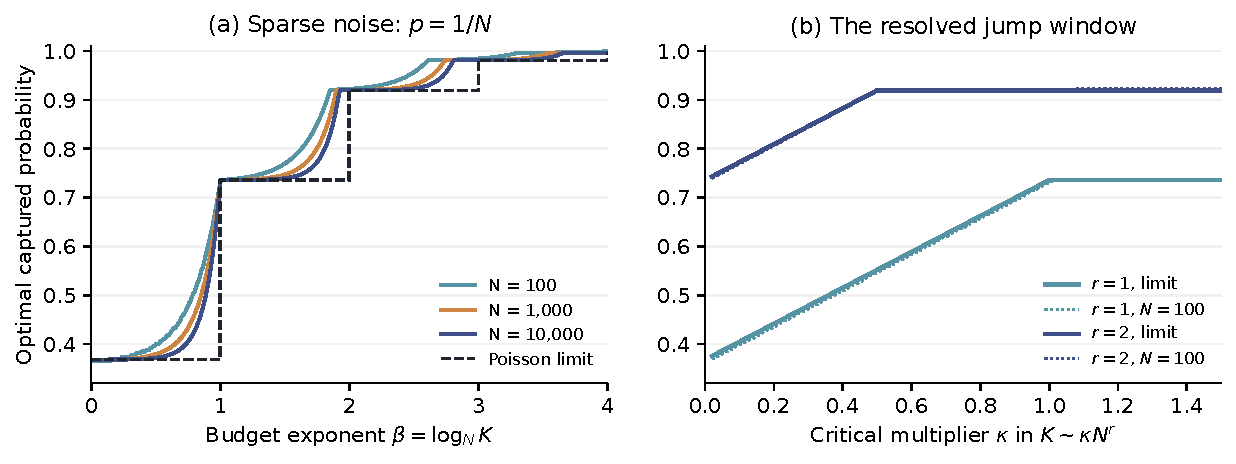
\includegraphics[width=0.97\textwidth]{figures/sparse_budget_staircase.pdf}
\caption{Exact finite optimal-catalog probabilities for sparse Bernoulli
noise with $p=1/N$. Left: the global polynomial-budget staircase; the dashed
curve is the Poisson limit. Right: the resolved critical multiplier at
$K\sim\kappa N^r$. Every curve is evaluated from the Hamming-layer formula;
no simulation of nonstandard arithmetic is involved.}
\label{fig:poisson}
\end{figure}

\begin{figure}[htbp]
\centering
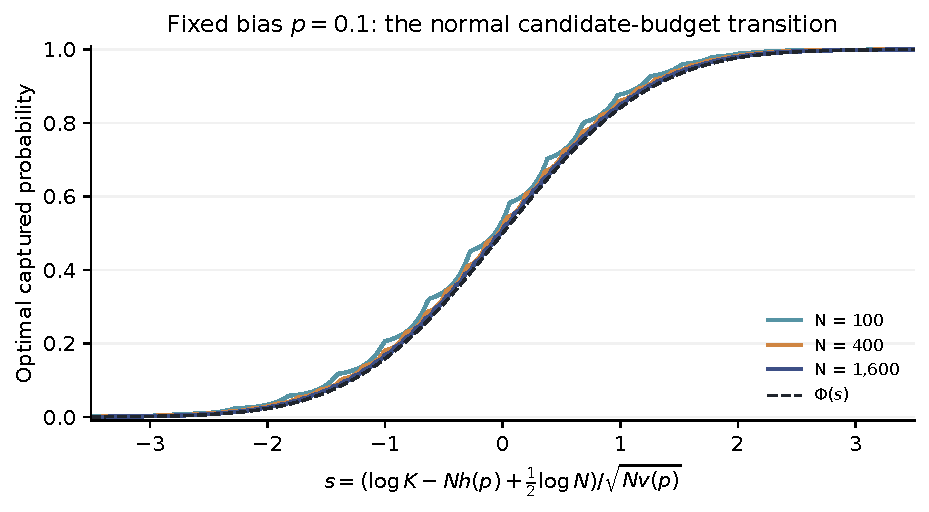
\includegraphics[width=0.80\textwidth]{figures/fixed_bias_normal_transition.pdf}
\caption{The fixed-bias normal transition. The standardized catalog budget
uses the entropy term, the square-root dispersion term, and the
$-\tfrac12\log N$ correction in Theorem~\ref{thm:budget-normal}.
Finite probabilities are computed from exact layer counts and numerical
binomial probabilities.}
\label{fig:normal}
\end{figure}

\begin{remark}[A fixed infinite law and a triangular array are different]
Theorem~\ref{thm:budget-atomic} concerns prefixes of one fixed infinite
sequence of biases. The sparse theorem uses a different product law at each
length $N$, with $p_N=\lambda/N$ at all of its sites. Bounded total row mass
in that triangular array does not imply uniformly bounded high-confidence
catalogs: for confidence above $e^{-\lambda}$, the budgets grow. There is
no contradiction with the summability theorem because no single infinite
bias sequence has those rows as all of its prefixes.
\end{remark}

\subsection{Why finite observations alone cannot certify noncoding}

There is a crucial limitation when transferring these finite budgets
back to a nonstandard arithmetic model.  If $x$ is nonstandard and
$\mathcal A_x$ is the external countable family of internally coded
binary words on $[0,x)$, then $\mathcal A_x$ realizes every prescribed
pattern on every externally finite subset of $[0,x)$.  Indeed one may
code the finitely many coordinates whose prescribed values are one and
give value zero elsewhere.  Thus $\mathcal A_x$ is dense in the external
product topology, even though in the nonsummable regime it has measure
zero.  No finite observation, including an adaptively selected finite
set of coordinates, can logically certify that a word is not internally
coded.  The finite candidate-budget problem is therefore an additional,
explicit resource restriction; its parameter $K$ must not be silently
identified with the full internal family of codes.




% ---- sections/outlook.tex ----
\section{Consequences linking the constructions}
\label{sec:consequences}

The universal construction has a stronger logical feature than arbitrary
coding cuts alone. Its Boolean outputs can be locally coded without
satisfying the stronger induction scheme.

\begin{corollary}[All nonconstant Boolean outputs fail stronger induction]
\label{cor:boolean-induction}
For a nonstandard $M$, in the realization of
Theorem~\ref{bs:universality}, and also in its vanishing-bias refinement,
almost surely every nonconstant finitary Boolean observable $R=f(P)$
fails $\mathsf I\Sigma_1(R)$. If its coding cut is $M$, it nevertheless
satisfies $\mathsf I\Delta_0(R,\E)$.
\end{corollary}

\begin{proof}
If the output cut is proper, use the bare-language coding formula from
Corollary~\ref{cor:induction-sigma-obstruction}. If its cut is $M$, consider
the deviation predicate $D$ from the all-zero output value $f(\mathbf0)$.
The proof of Theorem~\ref{bs:boolean} identifies its coding cut with the
summability cut of its deviation probabilities. Therefore every bounded
restriction of $D$ is externally finite almost surely. The marker
construction makes $D$ infinite almost surely, including in the
vanishing-bias refinement. Lemma~\ref{lem:induction-locally-finite} gives
failure of $\mathsf I\Sigma_1(D)$. If $R$ is the complement of $D$, literal
substitution of $\neg R$ for $D$ preserves the formula class and transfers
the failed induction instance. Complete local coding gives the bounded
induction statement. Countably many observables allow simultaneous
conclusions.
\end{proof}

\subsection{What the finite probabilities say about internal codes}

The finite optimization and the infinite classification use the same
mechanism at different quantifier scales. With independent coordinates,
the largest atom on a finite set $F$ is
\[
 \prod_{t\in F}(1-\varepsilon_t).
\]
If the accumulated minority mass diverges, this tends to zero. A fixed
finite catalog then loses all captured probability, and each individual
infinite word has probability zero. Countability of the internal catalog
is what turns that last statement into almost-sure noncoding.

When minority mass is summable, the observed infinite word is a finite
modification of its mode. A finite catalog can capture arbitrarily high
confidence uniformly in the observation length. Internal codability is
then determined by the modal word. These statements explain why the
infinite theorem is about minority-mass summability, whereas the
exponential growth rate of finite optimal catalogs is Shannon entropy.
The two quantities answer different questions and need not agree.

At sparse noise $p_N=\lambda/N$, the finite experiment retains a bounded
expected number of errors while their possible positions proliferate.
Naming all patterns with $r$ errors costs order $N^r$. That count produces
the Poisson staircase. It is a finite positional cost, even though the
number of errors has a tight limiting distribution.

For reference, the following values are obtained directly from the exact
finite formula at $N=10{,}000$ and $p=1/N$. They are numerical evaluations,
not experimental estimates from random trials.

\begin{center}
\begin{tabular}{lrr}
\toprule
Catalog size & Finite captured probability & Limiting probability\\
\midrule
$K=N/4$ & $0.45979872$ & $1.25/e\approx0.45984930$\\
$K=N$ & $0.73572209$ & $2/e\approx0.73575888$\\
$K=N^2/2$ & $0.91968940$ & $2.5/e\approx0.91969860$\\
\bottomrule
\end{tabular}
\end{center}

\section{A concrete formalization route in ProveIt}
\label{sec:formalization}

The mathematics naturally separates into interfaces that can be verified
independently and then connected. An efficient first target is the
single-predicate classification and its pairwise-independent extension;
the Boolean universality theorem can follow once the summability and
marker interfaces are available.

\subsection{Use raw first-order arithmetic semantics}

The inspected \texttt{NotFinitelyAxiomatizable} project explicitly works
with raw first-order arithmetic structures satisfying the $\PA$ schema
\cite{proveit-finite}. That distinction is essential. A host-level model
interface whose induction field ranges over \emph{all} ambient predicates
would exclude nonstandard models and would not express the setting here.

Its \texttt{FiniteBetaCoding.lean} proves that externally finite lists of
arbitrary elements of a raw $\PA$ model can be packed into beta codes
\cite{proveit-beta}. This addresses the important case in which a changed
bit position or a selected list entry is nonstandard. Its
\texttt{EvaluatorCutContract.lean} isolates an existing definable-cut
induction argument \cite{proveit-evaluator}; the present random coding
predicate needs a new contract, rather than an invocation of that theorem
with its evaluator hypotheses omitted.

The separate \texttt{ListCoding} README states a more limited formal
boundary for many exported formulas: their evaluation specifications are
metatheorems for the standard natural-number interpretation, not automatic
internal $\PA$ derivations of every universal closure \cite{proveit-list}.
Those results are useful starting points, but a theorem about arbitrary
nonstandard models must pass through the appropriate syntactic theorem and
soundness interfaces. The present report does not silently transfer
standard-model correctness to every model.

\subsection{Suggested proof modules}

\begin{longtable}{p{0.25\textwidth}p{0.67\textwidth}}
\toprule
Module or interface & Required statement and verification boundary\\
\midrule
\endfirsthead
\toprule
Module or interface & Required statement and verification boundary\\
\midrule
\endhead
Internal binary coding & Define the bit formula and prove restriction,
successor extension, Boolean closure, and externally finite modification
in arbitrary raw $\PA$ models. Record which facts are internal theorems
and which are external finite constructions.\\
Abstract coded traces & Package a countable family of patterns on each
initial interval, closed under finite changes and restriction. Prove the
cut and filtration lemmas without probability.\\
External summability & Use nonnegative-real sums or finite-subset suprema.
Prove successor closure, invariance under summable perturbations, and the
marker characterization. Do not substitute an internal arithmetic sum.\\
Probability classification & Prove the finite-tail implication, nullity
of a fixed trace, and the countable-code union. For pairwise independence,
verify the variance and second-moment bound separately.\\
Countable spectra & Formalize the enumeration of constraints and the
fresh-marker recursion. The decisive invariant controls all labels
containing a fixed finite set, not only one cofinal sequence.\\
Boolean observations & Compute minimal sensitive supports from a finite
truth table. Prove the disjoint-event lower bound and the union upper
bound before connecting their summability cuts.\\
Induction syntax & Construct the explicit bounded formula with $\E$ and
the bare-language beta formulas. Verify query bounds by recursion on
syntax; use arithmetic induction only after eliminating $P$ locally.\\
Finite catalogs & Certify the exchange argument, binomial-layer counts,
and quadratic dual bounds using exact rational arithmetic. The existing
Python checks are evidence for examples, not trusted proof objects.\\
\bottomrule
\end{longtable}

A formalization should expose theorem dependencies and avoid stating the
probabilistic conclusion as an axiom. The desired end product is an actual
proof that almost every predicate has the asserted coding cut, with the
countability assumptions visible in its type. Full formalization was not
performed in this report.

\section{Verification and source audit}
\label{sec:audit}

\subsection{Mathematical checks}

Independent derivations agreed on the arbitrary-bias formula, arbitrary-cut
realization, and the countable marker construction. A separate skeptical
review checked the Boolean comparisons, the weak-limit statement, the
beta-code conversion, and the induction phase diagram. The review produced
counterexamples to stronger but false formulations involving only marginal
fairness, only pairwise independence of array entries, independence of rows
without coordinate independence, or probabilities allowed to approach one.
The article states the narrower hypotheses that withstand these checks.
This is an internal research audit, not external peer review.

\subsection{Executed finite checks}

The included script \texttt{verify\_finite\_budgets.py} reproduces the
figures and CSV data and performs the following tests. The exact checks use
rational arithmetic and a second implementation that enumerates the
distribution's atoms.

\begin{center}
\begin{tabular}{p{0.69\textwidth}r}
\toprule
Check & Count\\
\midrule
Exact iid catalog formula versus sorted atom sums, $N\le10$ & $6{,}138$\\
Nonidentical-product projection and modal-extension bounds & $494$\\
Floating evaluation versus exact rational answers & $114$\\
Complete pairwise-independent extremizing distributions, $1\le N\le10$ & $10$\\
Exact fair-marginal identities in those distributions & $55$\\
Exact pairwise joint-probability identities & $660$\\
Pointwise quadratic majorant inequalities & $65$\\
Exact dual-expectation identities & $10$\\
\bottomrule
\end{tabular}
\end{center}

All checks passed. The maximum absolute error in the floating spot checks
was $3.33\times10^{-16}$. The generated JSON records the runtime versions,
counts, and scope. No finite structure was presented as a simulation of a
nonstandard model. The infinite results rest on the mathematical proofs,
and the tests establish neither those theorems nor historical priority.

\subsection{Source boundary}

Repository inspection used the pinned revision
\texttt{3b9458b31f459b480ab43a068d7cc56f4cfdbb28}. The focused files are
listed in the bibliography and in the package's source-audit text. Searches
for random predicates and coin flipping did not return an existing
repository treatment of the precise problem selected here. This focused
search is not an exhaustive audit of the entire repository or its incoming
archives.

The public Glazer source used for the direct research connection is the
official seminar abstract, not an inferred private preference. The
underlying video was not used as evidence for a particular formula.
The arithmetic-randomness theorem announced there, the established
source-coding asymptotics, and the known finite pairwise moment optimum
are explicitly credited. Our results are formulated so that their proofs
can be assessed independently of any priority claim.

\section{Further research questions and topics}
\label{sec:questions}

The following are proposed problems arising from this report. They are
not all asserted to be previously unposed problems in the literature.
Each entry identifies a concrete next target and the part of the present
work that makes it accessible.

\begin{enumerate}[label=\textbf{Q\arabic*.},leftmargin=*]
\item \textbf{The weakest arithmetic base.}
Determine the weakest arithmetic theory supporting the arbitrary-bias
classification and the countable conjunction universality theorem for one
uniform formula. The present proof uses total exponentiation and internal
binary coding in $\PA$. Glazer's announced fair-coin result reaches $Q$;
extending the full noise and Boolean classifications that far requires
an alternative to the coding operations assumed here. A first target is
an explicit elementary-arithmetic interface with all coding lemmas proved.

\item \textbf{Exact Borel complexity of cut fibers.}
Classify the exact Borel or Wadge complexity of $\mathcal E_I$ from the
order-theoretic position of $I$. The uniform $\Pi^0_3$ upper bound is
proved, and cuts with a cofinal successor block have lower-complexity
descriptions. Which remaining cuts attain the full bound? The closed-code
description and the finite two-limit representation give concrete
starting points for reductions.

\item \textbf{Automorphism-invariant laws.}
Which cuts can be selected by a law invariant under the automorphism
group of $M$? Such a cut must be invariant, but this necessary condition
need not provide biases whose local summability realizes it. The
arbitrary-marker construction deliberately makes no invariance demand.
Analyze orbit-constant biases first, then invariant dependent laws.

\item \textbf{Effective realization relative to a presentation.}
Given a presentation of a countable model and descriptions of its target
cuts, determine the oracle complexity needed to carry out the diagonal
marker construction. The existence proof enumerates all true constraints
$(S,a\in C_S)$ and is not an unconditional computable algorithm. An
oracle-relative construction, with explicit moduli for the finite
constraints, would connect the theorem to ProveIt's computability work.

\item \textbf{Arithmetic genericity under biased laws.}
Characterize the product measures that almost surely produce strongly
CP-generic predicates. The exact coding cut alone cannot encode all the
genericity requirements on definable tuples. Existing results rule out
strongly CP-generic classes in nonstandard models
\cite{abdul-quader-schmerl}; thus a maximal coding cut already supplies
an obstruction. Determine which additional divergence conditions on
definable families are sufficient and necessary.

\item \textbf{Induction over an arbitrary modal predicate.}
The exact cut formula allows an arbitrary modal pattern $b$, whereas
the three-regime full-induction theorem assumes zero-modal noise.
Classify higher induction in $(M,P)$ when the modal expansion $(M,b)$
has prescribed logical properties. Globally finite errors preserve
induction with parameters, but infinite locally finite errors may have
different effects when $b$ cannot itself be defined from $P$.

\item \textbf{Boolean spectra with correlations inside each site.}
Replace the product distribution across the input bits at a fixed site
by an arbitrary finite joint law, while keeping the vectors at different
sites independent. Determine the attainable Boolean cut tables. The
minimal-support rule in Theorem~\ref{bs:boolean} uses within-site
independence, and XOR cancellation shows it can fail without it. Finite
atom probabilities of these joint laws give a direct starting point.

\item \textbf{Quantitative approximate independence.}
The pairwise proof only needs the mismatch variance to be negligible
relative to the square of its mean along an exhaustion. Find useful
uniform conditions on covariance errors that guarantee this for all
internal codes simultaneously, and obtain optimal finite catalog bounds.
The exact estimate \eqref{eq:pairwise-mismatch} identifies the needed
scale; small pairwise errors individually may still accumulate too fast.

\item \textbf{More than one target under limited independence.}
For pairwise-independent fair bits and a specified catalog
$\mathcal C\subseteq\{0,1\}^N$, compute the exact maximum of
$\Prob(X\in\mathcal C)$. The atom optimum is known, but the bound
$Kq_N$ may lose information about overlaps and geometry for multiword
catalogs. Determine exact solutions for Hamming balls, linear catalogs,
and catalogs of two or three words before approaching arbitrary sets.

\item \textbf{All-order sparse expansions and inversion.}
Derive uniform higher-order expansions for $Q_N(K)$ and for the least
budget attaining a prescribed confidence when $p_N\to0$. The fixed
Poisson parameter, the transition $Np_N\to\infty$, lattice effects,
and a confidence approaching a staircase endpoint require different
scales. The exact Hamming-layer formula supplies a natural starting
point for asymptotic inversion and transseries methods.

\item \textbf{Algorithms for unequal biases.}
The exact optimum ranks subsets by sums of costs
$\log((1-\varepsilon_i)/\varepsilon_i)$. Determine efficient certified
algorithms for the first $K$ subsets, especially with many repeated or
structured biases. An arithmetic catalog imposed by a particular code
enumeration can be much harder than an unrestricted optimal list; the
computational resource model should make that distinction explicit.

\item \textbf{Growing or internally nonstandard alphabets.}
Finite fixed alphabets admit straightforward modal-probability variants
of the atom argument. The more interesting target is a uniform theory
when alphabet sizes grow, or when the model regards the alphabet itself
as nonstandard finite. How do finite-description costs, modal atoms,
and the complexity of a single coding formula interact then?

\item \textbf{A verified end-to-end theorem.}
Implement the arithmetic and probability interfaces of
Section~\ref{sec:formalization}, culminating first in
Theorem~\ref{thm:pairwise-cut}, then in
Theorem~\ref{bs:universality}. A meaningful deliverable would include a
kernel-checked countable-model theorem and independent finite certificates
for the source-coding and pairwise moment examples, with every unproved
interface stated separately.

\item \textbf{Beyond countable models.}
Determine replacements for the countable-null-union argument when the
family of internal codes is uncountable, and compare the relevant ideals
with those raised in Glazer's seminar. Standard systems, cardinal
invariants of null ideals, and local versus global measurability may
provide useful conditional statements. The present article makes no
claim about countably saturated uncountable models or their completed
product measures.
\end{enumerate}

The proposed problem is therefore solved at the level of arbitrary
single-predicate product laws and countable independent Boolean spectra
with biases uniformly bounded away from one,
with an exact finite catalog theory and several sharp limitations. Its
remaining questions concern symmetry, effective construction, weakened
arithmetic, and dependence: restrictions under which the freedom to
prescribe arbitrary cuts becomes a more rigid mathematical phenomenon.



% ---- sections/references.tex ----
\begin{thebibliography}{99}

\bibitem{glazer2023}
Elliot Glazer.
\emph{Coin flipping on models of arithmetic to define the standard cut}.
MOPA seminar, 17 October 2023. Official seminar abstract.
\url{https://nylogic.github.io/mopa/2023/10/17/coin-flipping-on-models-of-arithmetic-to-define-the-standard-cut.html}.
Accessed 5 October 2026.

\bibitem{abdul-quader-schmerl}
Athar Abdul-Quader and James H. Schmerl.
CP-generic expansions of models of Peano arithmetic.
\emph{Mathematical Logic Quarterly} \textbf{68} (2022), 171--177.
\href{https://doi.org/10.1002/malq.202100051}{doi:10.1002/malq.202100051}.
\url{https://arxiv.org/abs/2107.11867}.
The inspected preprint was version 3; its class obstruction is Theorem 19.

\bibitem{kontoyiannis-verdu}
Ioannis Kontoyiannis and Sergio Verd\'u.
Optimal lossless data compression: Non-asymptotics and asymptotics.
\emph{IEEE Transactions on Information Theory} \textbf{60}(2) (2014),
777--795.
\href{https://doi.org/10.1109/TIT.2013.2291007}{doi:10.1109/TIT.2013.2291007}.
Preprint: \emph{Lossless Data Compression at Finite Blocklengths},
\url{https://arxiv.org/abs/1212.2668}.

\bibitem{chen-effros-kostina}
Shuqing Chen, Michelle Effros, and Victoria Kostina.
Lossless source coding in the point-to-point, multiple access, and random
access scenarios.
\emph{IEEE Transactions on Information Theory} \textbf{66}(11) (2020),
6688--6722.
\href{https://doi.org/10.1109/TIT.2020.3005155}{doi:10.1109/TIT.2020.3005155}.
\url{https://arxiv.org/abs/1902.03366}.

\bibitem{benjamini-gurel-peled}
Itai Benjamini, Ori Gurel-Gurevich, and Ron Peled.
\emph{On K-wise Independent Distributions and Boolean Functions}.
arXiv:1201.3261, uploaded 2012; the abstract identifies an earlier
author-website manuscript. Proposition 25 gives the exact pairwise
atom formula used here.
\url{https://arxiv.org/abs/1201.3261}.

\bibitem{boros-prekopa}
Endre Boros and Andr\'as Pr\'ekopa.
Closed form two-sided bounds for probabilities that at least $r$ and
exactly $r$ out of $n$ events occur.
\emph{Mathematics of Operations Research} \textbf{14}(2) (1989), 317--342.
Bibliographic attribution and its application to pairwise independence
were checked in \cite{benjamini-gurel-peled}.

\bibitem{proveit-list}
Vladimir Reshetnikov, \emph{ProveIt},
\path{Logic/PeanoArithmetic/ListCoding/README.md}.
\href{https://github.com/VladimirReshetnikov/ProveIt/blob/3b9458b31f459b480ab43a068d7cc56f4cfdbb28/Logic/PeanoArithmetic/ListCoding/README.md}{Repository file at the inspected revision}.
Describes the formula interfaces and their standard-model verification
boundary. Accessed 5 October 2026.

\bibitem{proveit-finite}
Vladimir Reshetnikov, \emph{ProveIt},
\path{Logic/PeanoArithmetic/NotFinitelyAxiomatizable/README.md}.
\href{https://github.com/VladimirReshetnikov/ProveIt/blob/3b9458b31f459b480ab43a068d7cc56f4cfdbb28/Logic/PeanoArithmetic/NotFinitelyAxiomatizable/README.md}{Repository file at the inspected revision}.
Describes the raw-model, external finite coding, and definable-cut
architecture. Accessed 5 October 2026.

\bibitem{proveit-beta}
Vladimir Reshetnikov, \emph{ProveIt},
\path{PAFiniteBasisReduction/FiniteBetaCoding.lean}, under
\path{Logic/PeanoArithmetic/NotFinitelyAxiomatizable/Lean/}.
\href{https://github.com/VladimirReshetnikov/ProveIt/blob/3b9458b31f459b480ab43a068d7cc56f4cfdbb28/Logic/PeanoArithmetic/NotFinitelyAxiomatizable/Lean/PAFiniteBasisReduction/FiniteBetaCoding.lean}{Inspected Lean source}.
External finite beta coding in raw $\PA$ models. Accessed 5 October 2026.

\bibitem{proveit-evaluator}
Vladimir Reshetnikov, \emph{ProveIt},
\path{PAFiniteBasisReduction/EvaluatorCutContract.lean}, under
\path{Logic/PeanoArithmetic/NotFinitelyAxiomatizable/Lean/}.
\href{https://github.com/VladimirReshetnikov/ProveIt/blob/3b9458b31f459b480ab43a068d7cc56f4cfdbb28/Logic/PeanoArithmetic/NotFinitelyAxiomatizable/Lean/PAFiniteBasisReduction/EvaluatorCutContract.lean}{Inspected Lean source}.
The evaluator-independent definable-cut contract and induction argument.
Accessed 5 October 2026.

\end{thebibliography}



\end{document}
